\appendix
\renewcommand{\thechapter}{\Asbuk{chapter}} % использование русских букв для нумерации приложений
\selectlanguage{russian}

\chapter{Математическое приложение}\label{chap:discrete-math}

\section{Общие определения}

Выражением $\Mod n$ обозначается вычисление остатка от деления произвольного целого числа на целое число $n$. В полиномиальной арифметике эта операция означает вычисление остатка от деления многочленов.
%далее будем обозначать целые числа или операции с целыми числами, взятыми \emph{по модулю}\index{модуль} целого числа $n$ (остаток от целочисленного деления). Примеры выражений:
    \[ a\mod n, \]
    \[ (a + b)\cdot c\mod n. \]
Равенство
    \[ a = b \mod n \]
означает, что выражения $a$ и $b$ равны (говорят также <<сравнимы>>, <<эквивалентны>>) по модулю $n$.

Множество
    \[ \{ 0, 1, 2, 3, \dots, n-1 \mod n\} \]
состоит из $n$ элементов, где каждый элемент $i$ представляет все целые числа, сравнимые с $i$ по модулю $n$.

Наибольший общий делитель (НОД) двух чисел $a,b$ обозначается $\gcd(a,b)$ (\textit{greatest common divisor}).

Два числа $a,b$ называются взаимно простыми, если они не имеют общих делителей, кроме 1, то есть $\gcd(a,b) = 1$.

Выражение $a \mid b$ означает, что $a$ делит $b$.

\section{Парадокс дней рождения}\label{section-birthday-padradox}
\selectlanguage{russian}

Парадокс дней рождения\index{парадокс дней рождения} связан с контринтуитивным ответом на следующую задачу: какой должен быть минимальный размер группы, чтобы вероятность совпадения дней рождения хотя бы у пары человек из этой группы была больше $1 / 2$? Первый возникающий в голове вариант ответа <<183 человека>> (т.~е. $\left\lceil 365 / 2 \right\rceil$) является неверным.

Найдём вероятность $P(n)$ того, что в группе из $n$ человек хотя бы двое имеют день рождения в один день года. Вероятность того, что $n$ человек ($n < 365$) не имеют общего дня рождения, есть
\[
    \bar{P}(n) = 1 \cdot \left( 1 - \frac{1}{365} \right) \cdot \left(1 - \frac{2}{365} \right)  \dots  \left( 1 - \frac{n-1}{365} \right) = \prod\limits_{i=0}^{n-1} \left( 1 - \frac{i}{365} \right).
\]

Аппроксимируя $1-x \leq e^{-x}$, находим
    \[ \bar{P}(n) \approx \prod\limits_{i=0}^{n-1} e^{-\frac{i}{365}} = e^{-\frac{n(n-1)}{2} \cdot \frac{1}{365}} \approx e^{-\frac{n^2}{2} \cdot \frac{1}{365}}. \]

Вероятность того, что хотя бы 2 человека из $n$ имеют общий день рождения, есть
    \[ P(n) = 1 - \bar{P}(n) \approx 1 -  e^{-\frac{n^2}{2} \cdot \frac{1}{365}}. \]

Кроме того, найдём минимальный размер группы, в которой дни рождения совпадают хотя бы у двоих с вероятностью не менее $1/2$. То есть найдём такое число $n_{1/2}$, чтобы выполнялось условие $P(n_{1/2}) \geq \frac{1}{2}$. Подставляя это значение в формулу для вероятности, получим $\frac{1}{2} \geq e^{-\frac{n_{1/2}^2}{2} \cdot \frac{1}{365}}$. Следовательно,
	\[n_{1/2} \geq \sqrt{2 \ln 2 \cdot n} \approx 1,18 \sqrt{ n } \approx 22,5.\]
	
В криптографии при оценках стойкости алгоритмов часто опускают коэффициент $\sqrt{2 \ln 2}$, считая ответом на задачу <<округлённое>> значение $\sqrt{ n }$. Например, оценку числа операций хэширования для поиска коллизии идеальной криптографической хэш-функции с размером выхода k бит часто записывают как $2^{k/2}$.


\section{Группы}\label{section-groups}
\selectlanguage{russian}

\subsection{Свойства групп}

\textbf{Группой}\index{группа} называется множество $\Gr$, на котором задана бинарная операция <<$\cdot$>>, удовлетворяющая следующим аксиомам:
\begin{enumerate}
    \item замкнутость:
        \[ \forall a,b \in \Gr: a \cdot b = c \in \Gr; \]
    \item ассоциативность:
        \[ \forall a,b,c \in \Gr: (a \cdot b) \cdot c = a \cdot (b \cdot c); \]
    \item существование единичного элемента:
        \[ \exists ~ e \in \Gr: e\cdot a = a \cdot e = a; \]
    \item существование обратного элемента:
        \[ \forall a \in \Gr ~ \exists ~ b \in \Gr: a \cdot b = b \cdot a = e. \]
\end{enumerate}
Если
    \[ \forall a,b \in \Gr: a \cdot b = b \cdot a, \]
то группа коммутативная.

Если операция в группе задана как умножение <<$\cdot$>>, то группа называется \textbf{мультипликативной}, $e = 1$, обратный элемент -- $a^{-1}$, возведение в степень $k$ -- $a^k$.

Если операция задана как сложение <<$+$>>, то группа называется \textbf{аддитивной}, $e = 0$, обратный элемент $-a$, сложение $k$ раз -- $ka$.

Подмножество группы, удовлетворяющее аксиомам группы, называется \textbf{подгруппой}\index{подгруппа}.

\textbf{Порядком} $|\Gr|$ \textbf{группы}\index{порядок группы} $\Gr$ называется число элементов в группе. Пусть группа мультипликативная. Для любого элемента $a \in \Gr$ выполняется $a^{|\Gr|} = 1$.

\textbf{Порядком элемента} $a$ называется минимальное натуральное число
    \[ \ord(a): a^{\ord(a)} = 1. \]
 Порядок элемента делит порядок группы:
    \[ \ord(a) \mid \left|\Gr\right|. \]


\subsection{Циклические группы}

\textbf{Генератором} $g \in \Gr$ называется элемент, \emph{порождающий} всю группу\index{генератор группы}:
    \[ \Gr = \{g, g^2, g^3, \ldots, g^{|\Gr|} = 1\}. \]

Группа, в которой существует генератор, называется \textbf{циклической}\index{группа!циклическая}.

Если конечная группа не циклическая, то в ней существуют циклические подгруппы, порождённые всеми элементами. Любой элемент $a$ группы порождает либо циклическую \emph{подгруппу}
    \[ \{ a, a^2, a^3, \dots, a^{\ord(a)} = 1 \} \]
порядка $\ord(a)$, если порядок элемента $\ord(a) < |\Gr|$, либо \emph{всю} группу
    \[ \Gr = \{ a, a^2, a^3, \dots, a^{|\Gr|} = 1 \}, \]
если порядок элемента равен порядку группы $\ord(a) = |\Gr|$. Порядок любой подгруппы, как и порядок элемента, делит порядок всей группы.

Представим циклическую группу через генератор $g$ как
    \[ \Gr = \{g, g^2, \ldots, g^{|\Gr|} = 1\} \]
и каждый элемент $g^i$ возведём в степени $1, 2, \ldots, |\Gr|$. Тогда
\begin{itemize}
    \item элементы $g^i$, для которых число $i$ взаимно просто с $|\Gr|$, породят снова всю группу
            \[ \Gr = \{ g^i, g^{2i}, g^{3i}, \dots, g^{|\Gr| i} = 1 \}, \]
        так как степени $\{i, 2i, 3i, \dots, |\Gr| i \}$ по модулю $|\Gr|$ образуют перестановку чисел $\{1, 2, 3, \dots, |\Gr|\}$; следовательно $g^i$ -- тоже генератор, число таких чисел $i$ по определению функции Эйлера $\varphi(|\Gr|)$ ($\varphi(n)$ -- количество взаимно простых с $n$ целых чисел в диапазоне $[1,n-1]$);
    \item элементы $g^i$, для которых $i$ имеют общие делители
            \[ d_i = \gcd(i, |\Gr|) \neq 1 \]
        c $|\Gr|$, породят подгруппы
            \[ \{ g^i, g^{2i}, g^{3i}, \dots, g^{\frac{i}{d_i} |\Gr|} = 1\}, \]
        так как степень последнего элемента кратна $|\Gr|$; следовательно такие $g^i$ образуют циклические подгруппы порядка $d_i$.
\end{itemize}

Из предыдущего утверждения следует, что число генераторов в циклической группе равно
    \[ \varphi(|\Gr|). \]

Для проверки, является ли элемент генератором всей группы, требуется знать разложение порядка группы $|\Gr|$ на множители. Далее элемент возводится в степени, равные всем делителям порядка группы, и сравнивается с единичным элементом $e$. Если ни одна из степеней не равна $e$, то этот элемент является примитивным элементом или генератором группы. В противном случае элемент будет генератором какой-либо подгруппы.

Задача разложения числа на множители является трудной для вычисления. На сложности её решения, например, основана криптосистема RSA\index{криптосистема!RSA}. Поэтому при создании больших групп желательно заранее знать разложение порядка группы на множители для возможности выбора генератора.


\subsection{Группа $\Z_p^*$}\label{section-group-multiplicative}

\textbf{Группой $\Z_p^*$} называется группа\index{группа!$\Z_p^*$}
    \[ \Z_p^* = \{1, 2, \dots, p-1 \mod p\}, \]
где $p$ -- простое\index{число!простое} число, операция в группе -- умножение $\ast$ по $\mod p$.

Группа $\Z_p^*$ -- \textbf{циклическая}, порядок
    \[ |\Z_p^*| = \varphi(p) = p - 1. \]
Число генераторов в группе --
    \[ \varphi(|\Z_p^*|) = \varphi(p-1). \]

Из того, что $\Z_p^*$ -- группа, для простого\index{число!простое} $p$ и любого $a \in [2, p-1] \mod p$ следует \textbf{малая теорема Ферма}\index{теорема!Ферма малая}:
    \[ a^{p-1} = 1 \mod p. \]
На малой теореме Ферма основаны многие тесты проверки числа на простоту.

\example 1
Рассмотрим группу $\Z_{19}^*$. Порядок группы -- 18. Делители: 2, 3, 6, 9. Является ли 12 генератором?
\[ \begin{array}{l}
    12^2 = -8 \mod 19, \\
    12^3 = -1 \mod 19, \\
    12^6 = 1 \mod 19, \\
\end{array} \]
12 -- генератор подгруппы 6 порядка. Является ли 13 генератором?
\[ \begin{array}{l}
    13^2 = -2 \mod 19, \\
    13^3 = -7 \mod 19, \\
    13^6 = -8 \mod 19, \\
    13^9 = -1 \mod 19, \\
    13^{18} = 1 \mod 19, \\
\end{array} \]
13 -- генератор всей группы.
\exampleend

\example 2
В таблице~\ref{tab:Zp-sample} приведён пример группы $\Z_{13}^*$. Число генераторов -- $\varphi(12) = 4$. Подгруппы --
    \[ \Gr^{(1)}, \Gr^{(2)}, \Gr^{(3)}, \Gr^{(4)}, \Gr^{(6)}, \]
верхний индекс обозначает порядок подгруппы.

\begin{table}[!ht]
    \centering
    \caption {Генераторы и циклические подгруппы группы $\Gr=\Z_{13}^*$\label{tab:Zp-sample}}
    \resizebox{\textwidth}{!}{ \begin{tabular}{|c|p{0.66\textwidth}|c|}
        \hline
        Элемент & Порождаемая группа или подгруппа & Порядок \\
        \hline
         1 & $\Gr^{(1)} = \{  1 \}$ & 1 \\
         2 & $\Gr = \{ 2, 4, 8, 3, 6, 12, 11, 9, 5, 10, 7, 1 \}$ & 12, ген. \\
         3 & $\Gr^{(3)} = \{ 3, 9, 1 \}$ & 3 \\
         4 & $\Gr^{(6)} = \{ 4, 3, 12, 9, 10, 1 \}$ & 6 \\
         5 & $\Gr^{(4)} = \{ 5, 12, 8, 1 \}$ & 4 \\
         6 & $\Gr = \{ 6, 10, 8, 9, 2, 12, 7, 3, 5, 4, 11, 1 \}$ & 12, ген. \\
         7 & $\Gr = \{ 7, 10, 5, 9, 11, 12, 6, 3, 8, 4, 2, 1 \}$ & 12, ген. \\
         8 & $\Gr^{(4)} = \{ 8, 12, 5, 1 \}$ & 4 \\
         9 & $\Gr^{(3)} = \{ 9, 3, 1 \}$ & 3 \\
        10 & $\Gr^{(6)} = \{ 10, 9, 12, 3, 4, 1 \}$ & 6 \\
        11 & $\Gr = \{ 11, 4, 5, 3, 7, 12, 2, 9, 8, 10, 6, 1 \}$ & 12, ген. \\
        12 & $\Gr^{(2)} = \{ 12, 1 \}$ & 2 \\
        \hline
    \end{tabular} }
\end{table}
\exampleend


\subsection{Группа $\Z_n^*$}

\textbf{Функция Эйлера}\index{функция!Эйлера} $\varphi(n)$ определяется как количество чисел, взаимно простых с $n$ в интервале от 1 до $n-1$.

Если $n=p$ -- простое\index{число!простое} число, то
    \[ \varphi(p) = p - 1, \]
    \[ \varphi(p^k) = p^k - p^{k-1} = p^{k-1}(p - 1). \]
Если $n$ -- составное число и
    \[ n = \prod \limits_{i} p_i^{k_i} \]
разложено на простые множители $p_i$, то
    \[ \varphi(n) = \prod \limits_{i} \varphi(p_i^{k_i}) =  \prod \limits_{i} p_i^{k_i - 1}(p_i - 1). \]

\textbf{Группой $\Z_n^*$} называется группа\index{группа!$\Z_n^*$}
    \[ \Z_n^* = \left\{ \forall a \in \left\{ 1, 2, \dots, n-1 \mod n \right\} : \gcd(a,n) = 1 \right\} \]
с операцией умножения $\ast$ по $\mod n$.

Порядок группы --
    \[ |\Z_n^*| = \varphi(n). \]
Группа $\Z_p^*$ -- частный случай группы $\Z_n^*$.

Если $n$ \emph{составное}\index{число!составное} (не простое) число, то группа $\Z_n^*$ \textbf{нециклическая}.

Из того, что $\Z_n^*$ -- группа, для любых $a \neq 0, n > 1: \gcd(a,n) = 1$ следует \textbf{теорема Эйлера}\index{теорема!Эйлера}:
    \[ a^{\varphi(n)} = 1 \mod n. \]

При возведении в степень, если $\gcd(a,n) = 1$, выполняется
    \[ a^b = a^{b \mod \varphi(n)} \mod n. \]

\example
В таблице~\ref{tab:Zn-sample} приведена нециклическая группа $\Z_{21}^*$ и её циклические подгруппы
    \[ \Gr^{(1)}, \Gr_1^{(2)}, \Gr_2^{(2)}, \Gr_3^{(2)}, \Gr_1^{(3)}, \Gr_1^{(6)}, \Gr_2^{(6)}, \Gr_3^{(6)}, \]
верхний индекс обозначает порядок подгруппы, нижний индекс нумерует различные подгруппы одного порядка.

\begin{table}[!ht]
    \centering
    \caption{Циклические подгруппы нециклической группы $\Z_{21}^*$\label{tab:Zn-sample}}
    \begin{tabular}{|c|l|c|}
        \hline
        Элемент & Порождаемая циклическая подгруппа & Порядок \\
        \hline
        1  & $\Gr^{(1)} = \{ 1 \}$ & 1 \\
        2  & $\Gr_1^{(6)} = \{ 2, 4, 8, 16, 11, 1 \}$ & 6 \\
        4  & $\Gr_1^{(3)} = \{ 4, 16, 1 \}$ & 3 \\
        5  & $\Gr_2^{(6)} = \{ 5, 4, 20, 16, 17, 1 \}$ & 6 \\
        8  & $\Gr_1^{(2)} = \{ 8, 1 \}$ & 2 \\
        10 & $\Gr_3^{(6)} = \{ 10, 16, 13, 4, 19, 1 \}$ & 6 \\
        11 & $\Gr_1^{(6)} = \{ 11, 16, 8, 4, 2, 1 \}$ & 6 \\
        13 & $\Gr_2^{(2)} = \{ 13, 1 \}$ & 2 \\
        16 & $\Gr_1^{(3)} = \{ 16, 4, 1 \}$ & 3 \\
        17 & $\Gr_2^{(6)} = \{ 17, 16, 20, 4, 5, 1 \}$ & 6 \\
        19 & $\Gr_3^{(6)} = \{ 19, 4, 13, 16, 10, 1 \}$ & 6 \\
        20 & $\Gr_3^{(2)} = \{ 20, 1 \}$ & 2 \\
        \hline
    \end{tabular}
\end{table}
\exampleend

\subsection{Конечные поля}\label{section-fields}

\textbf{Полем} называется множество $\F$, для которого\index{поле}:
\begin{itemize}
    \item заданы две бинарные операции, условно называемые операциями умножения <<$\cdot$>> и сложения <<$+$>>;
    \item выполняются аксиомы группы для операции <<сложения>>: \\
        1. Замкнутость:
		\[\forall a, b \in \F: a + b \in \F.\]
        2. Ассоциативность:
		\[\forall a, b, c \in \F: (a+b)+c = a+(b+c).\]
        3. Существование нейтрального элемента по сложению (часто обозначаемого как <<0>>):
		\[\exists 0 \in \F: \forall a \in \F: a + 0 = 0 + a = a. \]
        4. Cуществование обратного элемента:
		\[\forall a \in \F: \exists -a: a + (-a) = 0. \]
    \item выполняются аксиомы группы для операции <<умножения>>, за одним исключением: \\
        1. Замкнутость:
		\[\forall a, b \in \F: a \cdot b \in \F. \]
        2. Ассоциативность:
		\[\forall a, b, c \in \F: (a \cdot b) \cdot c = a \cdot (b \cdot c).\]
        3. Существование нейтрального элемента по умножению (часто обозначаемого как <<1>>):
		\[\exists 1 \in \F: \forall a \in \F: a \cdot 1 = 1 \cdot a = a.\]
        4. Существование обратного элемента по умножению для всех элементов множества, кроме нейтрального элемента по сложению:
		\[\forall a \in {\F \backslash 0}: \exists a^{-1}: a \cdot a^{-1} = a^{-1} \cdot a = 1.\]
    \item операции <<сложения>> и <<умножения>> коммутативны: \\
        \[ \begin{array}{l}
            \forall a, b \in \F: a + b = b + a, \\
            \forall a, b \in \F: a \cdot b = b \cdot a; \\
        \end{array} \]
    \item выполняется свойство дистрибутивности:
        \[ \forall a, b, c \in \F: a \cdot (b + c) = (a \cdot b) + (a \cdot c). \]
\end{itemize}

Примеры \emph{бесконечных} полей (с бесконечным числом элементов): поле рациональных чисел $\group{Q}$, поле вещественных чисел $\group{R}$, поле комплексных чисел $\group{C}$ с обычными операциями сложения и умножения.

В криптографии рассматриваются \emph{конечные} поля (с конечным числом элементов), называемые также \textbf{полями Галуа}.

Число элементов в любом конечном поле равно $p^n$, где $p$ -- простое\index{число!простое} число и $n$ -- натуральное число. Обозначения поля Галуа: $\GF{p}, \GF{p^n}, \F_p, \F_{p^n}$ (аббревиатура от Galois field). Все поля Галуа $\GF{p^n}$ изоморфны друг другу (существует взаимно однозначное отображение между полями, сохраняющее действие всех операций). Другими словами, существует только одно поле Галуа $\GF{p^n}$ для фиксированных $p, n$.

Приведём примеры конечных полей.

Двоичное поле $\GF{2}$ состоит из двух элементов. Однако задать его можно разными способами:
\begin{itemize}
	\item Как множество из двух чисел <<0>> и <<1>> с определёнными на нём операциями <<сложение>> и <<умножение>> как сложение и умножение чисел по модулю 2. Нейтральным элементом по сложению будет <<0>>, по умножению -- <<1>>:
\[\begin{array}{ll}
	0 + 0 = 0,	& 	0 \cdot 0 = 0, \\
	0 + 1 = 1,	& 	0 \cdot 1 = 0, \\
	1 + 0 = 1,	& 	1 \cdot 0 = 0, \\
	1 + 1 = 0,	& 	1 \cdot 1 = 1. \\
\end{array}\]
	\item Как множество из двух логических объектов <<ЛОЖЬ>> ($F$) и <<ИСТИНА>> ($T$) с определёнными на нём операциями <<сложение>> и <<умножение>> как булевые операции <<исключающее или>> и <<и>> соответственно. Нейтральным элементом по сложению будет <<ЛОЖЬ>>, по умножению -- <<ИСТИНА>>:
\[\begin{array}{ll}
	F + F = F,	& 	F \cdot F = F, \\
	F + T = T,	& 	F \cdot T = F, \\
	T + F = T,	& 	T \cdot F = F, \\
	T + T = F,	& 	T \cdot T = T. \\
\end{array}\]
	\item Как множество из двух логических объектов <<ЛОЖЬ>> ($F$) и <<ИСТИНА>> ($T$) с определёнными на нём операциями <<сложение>> и <<умножение>> как булевые операции <<эквивалентность>> и <<или>> соответственно. Нейтральным элементом по сложению будет <<ИСТИНА>>, по умножению -- <<ЛОЖЬ>>:
\[\begin{array}{ll}
	F + F = T,	& 	F \cdot F = F, \\
	F + T = F,	& 	F \cdot T = T, \\
	T + F = F,	& 	T \cdot F = T, \\
	T + T = T,	& 	T \cdot T = T. \\
\end{array}\]
	\item Как множество из двух чисел <<0>> и <<1>> с определёнными на нём операциями <<сложение>> и <<умножение>>, заданными в табличном представлении. Нейтральным элементом по сложению будет <<1>>, по умножению -- <<0>>:
\[\begin{array}{ll}
	0 + 0 = 1,	& 	0 \cdot 0 = 0, \\
	0 + 1 = 0,	& 	0 \cdot 1 = 1, \\
	1 + 0 = 0,	& 	1 \cdot 0 = 1, \\
	1 + 1 = 1,	& 	1 \cdot 1 = 1. \\
\end{array}\]
\end{itemize}

Все перечисленные выше варианты множеств изоморфны друг другу. Поэтому в дальнейшем под конечным полем $\GF{p}$, где $p$ -- простое\index{число!простое} число, будем понимать поле, заданное как множество целых чисел от $0$ до $p-1$ включительно, на котором операции <<сложение>> и <<умножение>> заданы как операции сложения и умножения чисел по модулю числа $p$. Например, поле $\GF{7}$ будем считать состоящим из 7-ми чисел $\{0, 1, 2, 3, 4, 5, 6\}$ с операциями умножения $(\cdot \mod 7)$ и сложения $(+ \mod 7)$ по модулю.

Конечное поле $\GF{p^n}, n > 1$ строится \textbf{расширением} \emph{базового} поля $\GF{p}$. Элемент поля представляется как многочлен степени $n-1$ (или меньше) с коэффициентами из базового поля $\GF{p}$:
    \[ \alpha = \sum\limits_{i=0}^{n-1} a_i x^i, ~ a_i \in \GF{p}. \]

Операция сложения элементов в таком поле традиционно задаётся как операция сложения коэффициентов при одинаковых степенях в базовом поле $\GF{p}$. Операция умножения -- как умножение многочленов со сложением и умножением коэффициентов в базовом поле $\GF{p}$ и дальнейшим приведением результата по модулю некоторого заданного (для поля) неприводимого\footnote{Многочлен называется \textbf{неприводимым}\index{многочлен!неприводимый}, если он не раскладывается на множители, и \textbf{приводимым}\index{многочлен!приводимый}, если раскладывается.} многочлена $m(x)$. Количество элементов в поле равно $p^n$.

Многочлен $g(x)$ называется \textbf{примитивным элементом}\index{многочлен!примитивный} (генератором) поля, если его степени порождают все ненулевые элементы, то есть $\GF{p^n} \setminus \{0\}$, заданное неприводимым многочленом $m(x)$, за исключением нуля:
    \[ \GF{p^n} \setminus \{0\} = \{ g(x), g^2(x), g^3(x), \dots, g^{p^n-1}(x) = 1 \mod m(x) \}. \]

\example
В таблице~\ref{tab:irreducible-gf2} приведены примеры многочленов \emph{над полем} $\GF{2}$.
\begin{table}[!ht]
    \centering
    \caption{Пример многочленов над полем $\GF{2}$\label{tab:irreducible-gf2}}
    \begin{tabular}{|c|c|c|}
        \hline
        Многочлен & \parbox{2.5cm}{Упрощённая запись} & Разложение \\
        \hline
        $'1' x + '0'$ & $x$ & неприводимый \\
        $'1' x + '1'$ & $x+1$ & неприводимый \\
        $'1' x^2 + '0' x + '0'$ & $x^2$ & $x \cdot x$ \\
        $'1' x^2 + '0'x + '1'$ & $x^2 + 1$ & $(x+1) \cdot (x+1)$ \\
        $'1' x^2 + '1' x + '0'$ & $x^2 + x$ & $x \cdot (x+1)$ \\
        $'1' x^2 + '1' x + '1'$ & $x^2 + x + 1$ & неприводимый \\
        $'1' x^3 + '0' x^2 + '0' x + '1'$ & $x^3 + 1$ & $(x+1) \cdot (x^2+x+1)$ \\
        \hline
    \end{tabular}
\end{table}
\exampleend


\section{Конечные поля и операции в алгоритме AES}
\selectlanguage{russian}

В алгоритме блокового шифрования AES преобразования над байтами и битами осуществляются специальными математическими операциями. Биты и байты понимаются как элементы поля.

\subsection{Определение поля Галуа}

%Группой называется множество $\Gr$, в котором задана операция $\centerdot$ между двумя элементами группы и удовлетворяются аксиомы:
%\begin{enumerate}
%    \item Замкнутость -- $\forall a,b \in \Gr: a \centerdot b = c \in \Gr$.
%    \item Ассоциативность -- $\forall a,b,c \in \Gr: (a \centerdot b) \centerdot c = a \centerdot (b \centerdot c)$.
%    \item Существование единичного элемента -- $\exists ~ e \in \Gr: e\centerdot a = a \centerdot e = a$.
%    \item Существование обратного элемента -- $\forall a \in \Gr ~ \exists ~ b \in \Gr: a \centerdot b = b \centerdot a = e$.
%\end{enumerate}

\textbf{Полем} называется множество $\F$, для которого\index{поле}
\begin{itemize}
    \item заданы операции умножения <<$\cdot$>> и сложения <<$+$>>;
    \item выполняются аксиомы группы по сложению <<$+$>> для всего множества $\F$: \\
        1. для $a,b,c \in \F$ верно $a+b \in \F$, \\
        2. $(a+b)+c = a+(b+c)$, \\
        3. существует нулевой элемент -- ноль 0, $a+0=0+a=a$, \\
        4. существует единственный обратный элемент $-a$: \\
        \indent \indent \indent ~~~~~~ $a + (-a) = (-a) + a = 0$;
    \item выполняются аксиомы группы по умножению <<$\cdot$>> для множества $\{ \F \backslash 0 \}$, за исключением нуля: \\
        1. для $a,b,c \in \{ \F \backslash 0 \}$ верно \\
        \indent \indent \indent ~~~~~~ $a \cdot b \in \{ \F \backslash 0 \}$, \\
        \indent \indent \indent ~~~~~~ $(a \cdot b) \cdot c = a \cdot (b \cdot c)$, \\
        2. существует единичный элемент -- единица 1, ~ $a \cdot 1 = 1 \cdot a = a$, \\
        3. существует единственный обратный элемент $a^{-1}:$ \\
        \indent \indent \indent ~~~~~~ $a \cdot a^{-1} = a^{-1} \cdot a = 1$, \\
        к нулю 0 не существует обратного элемента и $a \cdot 0 = 0$;
%    \item Удовлетворяющее аксиомам группы по сложению и умножению, обратный элемент по умножению существует ко всем элементам кроме 0.
    \item операции сложения и умножения коммутативны
        \[ \begin{array}{l}
            a + b = b + a, \\
            a \cdot b = b \cdot a; \\
        \end{array} \]
    \item выполняется свойство дистрибутивности
        \[ a \cdot (b + c) = (a \cdot b) + (a \cdot c). \]
\end{itemize}

Примеры \emph{бесконечных} полей (с бесконечным числом элементов) -- поле рациональных чисел $\group{Q}$, поле вещественных чисел $\group{R}$, поле комплексных чисел $\group{C}$ с обычными операциями сложения и умножения.

В криптографии рассматриваются \emph{конечные} поля (с конечным числом элементов), называемые также \textbf{полями Галуа}.

Число элементов в любом конечном поле равно $p^n$, где $p$ -- простое число и $n$ -- натуральное число. Обозначения поля Галуа: $\GF{p}, \GF{p^n}, \F_p, \F_{p^n}$ (аббревиатура от Galois field). Все поля Галуа $\GF{p^n}$ изоморфны друг другу (существует взаимно однозначное отображение между полями, сохраняющее действие всех операций). Другими словами, существует только одно поле Галуа $\GF{p^n}$ для фиксированных $p, n$.

Приведем примеры конечных полей.

Двоичное поле $\GF{2}$ состоит из двух элементов:
    \[ \GF{2} = \{0, 1\} \]
с операцией $(\cdot)$ обычного умножения и сложения  $\oplus$ по модулю 2 (исключающее ИЛИ, XOR).

Поле
    \[ \GF{3} = \{0, 1, 2\} \]
состоит из 3-х элементов с операциями умножения $(\cdot \mod 3)$ и сложения $(+ \mod 3)$ по модулю.

Двоичное поле $\GF{2^n}$ строится \textbf{расширением} \emph{базового} поля $\GF{2}$. Элемент поля задается многочленом степени $n-1$ (или меньше) с коэффициентами из базового поля $\GF{2}$:
    \[ \alpha = \sum\limits_{i=0}^{n-1} a_i x^i, ~ a_i \in \GF{2}. \]
Сложение многочленов -- сложение коэффициентов при одинаковых степенях $x^i$ в поле $\GF{2}$, т.е. по $\text{XOR}$. Умножение многочленов в поле -- обычное умножение многочленов со сложением и умножением коэффициентов в поле $\GF{2}$ и дальнейшим приведением результата по модулю неприводимого многочлена $m(x)$ над полем $\GF{2}$.

Многочлен над базовым полем $\GF{p}$ называется \textbf{неприводимым}\index{многочлен!неприводимый}, если он не раскладывается на множители, и \textbf{приводимым}\index{многочлен!приводимый}, если раскладывается на множители.

Говорят, что неприводимый над базовым полем $\GF{p}$ многочлен $m(x)$ степени $n$ задает поле $\GF{p^n}$, если операция умножения в поле определена по модулю $m(x)$ (сложение определяется базовым полем, умножение -- многочленом $m(x)$). Количество элементов в поле определяется степенью $m(x)$) и равно $p^n$. Элементы поля есть остатки от деления на $m(x)$ и имеют степень не выше $n-1$.

Многочлен $g(x)$ называется \textbf{примитивным элементом}\index{многочлен!примитивный} (генератором) поля, если его степени порождают все ненулевые элементы, т.е. $\{ \GF{p^n} ~\backslash~ 0 \}$, заданное неприводимым многочленом $m(x)$, за исключением нуля:
    \[ \{ \GF{p^n} ~\backslash~ 0 \} = \{~ g(x), ~g^2(x), ~g^3(x),  \dots,  g^{p^n-1}(x) = 1 \mod m(x) ~\}. \]

Неприводимый многочлен $\mod m(x)$ называется  \textbf{примитивным}\index{многочлен!примитивный}, если $g(x)=x$.

\example
В табл. \ref{tab:irreducible-gf2} приведены примеры многочленов \emph{над полем} $\GF{2}$.
\begin{table}[h!]
    \centering
    \caption{Пример многочленов над полем $\GF{2}$\label{tab:irreducible-gf2}}
    \begin{tabular}{|c|c|c|}
        \hline
        Многочлен & \parbox{2.5cm}{Упрощенная запись} & Разложение \\
        \hline
        $'1' x + '0'$ & $x$ & неприводимый \\
        $'1' x + '1'$ & $x+1$ & неприводимый \\
        $'1' x^2 + '0' x + '0'$ & $x^2$ & $x \cdot x$ \\
        $'1' x^2 + '0'x + '1'$ & $x^2 + 1$ & $(x+1) \cdot (x+1)$ \\
        $'1' x^2 + '1' x + '0'$ & $x^2 + x$ & $x \cdot (x+1)$ \\
        $'1' x^2 + '1' x + '1'$ & $x^2 + x + 1$ & неприводимый \\
        $'1' x^3 + '0' x^2 + '0' x + '1'$ & $x^3 + 1$ & $(x+1) \cdot (x^2+x+1)$ \\
        \hline
    \end{tabular}
\end{table}
\exampleend


\subsection{Операции с байтами в AES}

Чтобы определить операции сложения и умножения двух байтов, введем сначала представление байта в виде многочлена степени 7 или меньше. Байт
    \[ a =( a_7, a_6, a_5, a_4, a_3, a_2, a_1, a_0) \]
преобразуется в многочлен $a(x)$ с коэффициентами 0 или 1 по правилу
    \[ a(x) = a_{7}x^{7}+a_{6}x^{6}+a_{5}x^{5}+a_{4}x^{4}+a_{3}x^{3}+a_{2}x^{2}+a_{1}x+a_{0}. \]

Далее байт трактуется как элемент конечного поля $\GF{2^8}$, заданного неприводимым многочленом
    \[ m(x) = x^{8}+x^{4}+x^{3}+x +1. \]

Произведение многочленов $a(x)$ и $b(x)$  по модулю многочлена $m(x)$  записывают как
    \[ c(x) = a(x) b(x) \mod m(x). \]
Остаток $c(x)$ представляет собой многочлен степени 7 или меньше. Его коэффициенты $(c_{7}, c_{6}, c_{5}, c_{4}, c_{3}, c_{2}, c_{1}, c_{0})$ образуют байт $c$, который и называется произведением байтов $a$ и $b$.

Сложение байтов осуществляется по $\oplus$ (исключающее ИЛИ), что является операцией сложения многочленов в двоичном поле.

\emph{Единичным} элементом поля является байт 00000001, или $\mathrm{'01'}$ в шестнадцатеричной записи. \emph{Нулевым} элементом поля является байт 00000000, или $\mathrm{'00'}$ в шестнадцатеричной записи. Одним из \emph{примитивных} элементов поля является байт (0 0 0 0 0 0 1 0), или $\mathrm{'02'}$ в шестнадцатеричной записи. Байты часто записывают в шестнадцатеричной форме, но при математических преобразованиях они должны интерпретироваться как элементы поля $\GF{2^8}$.

Для каждого ненулевого байта $a$ существует обратный байт $b$, такой, что их произведение является единичным байтом:
    \[ a b = 1 \mod m(x). \]
Обратный байт обозначается $b = a^{-1}$.

Для байта $a$, представленного многочленом $a(x)$, нахождение обратного байта $a^{-1}$ сводится к решению уравнения
    \[ m(x) d(x) + b(x) a(x) = 1. \]
Если такое решение найдено, то многочлен $b(x) \mod m(x)$ является представлением обратного байта $a^{-1}$. Обратный элемент (байт) может быть найден с помощью расширенного алгоритма Евклида для многочленов.

\example
Найти байт, обратный байту $a = \mathrm{'83'}$ в шестнадцатеричной записи. Так как $a(x) = x^{7} + x^{6} + 1$, то с помощью расширенного алгоритма Евклида находим
    \[ (x^{8} + x^{4} + x^{3} + x + 1) (x^{4} + x^{3} + x^{2} + x + 1) + (x^{7} + x^{6} + 1) (x^{5} + x^{3}) = 1. \]
Таким образом, обратный элемент поля или обратный байт $\mathrm{'83'}$ равен
    \[ x^{5} + x^{3}, ~ a^{-1} = \mathrm{'00101000'} = \mathrm{'28'}. \]
\exampleend

\example
В алгоритме блокового шифрования AES байты рассматриваются как элементы поля Галуа $\GF{2^8}$. Сложим байты $\mathrm{'57'}$ и $\mathrm{'83'}$. Представляя их многочленами, находим
    \[ (x^6 + x^4 + x^2 + x + 1) + (x^7 + x + 1) = x^7 + x^6 + x^4 + x^2, \]
или в двоичной записи --
    \[ 01010111 \oplus 10000011 = 11010100 = \mathrm{'D4'}. \]
Получили $\mathrm{'57'} + \mathrm{'83'} = \mathrm{'D4'}$.
\exampleend

\example
Выполним в поле $\GF{2^8}$, заданном неприводимым многочленом
    \[ m(x) = x^8 + x^4 + x^3 + x + 1 \]
(из алгоритма AES) операции с байтами: $\mathrm{'FA'} \cdot \mathrm{'A9'} + \mathrm{'E0'}$:
    \[ FA = 11111010, ~ A9 = 10101001, ~ E0 = 11100000, \]
    \[ (x^7 + x^6 + x^5 + x^4 + x^3  +x)(x^7 + x^5 + x^3 + 1) + (x^7 + x^6 + x^5) \mod m(x) = \]
    \[ = x^{14} + x^{13} + x^{10} + x^{8} + x^7 + x^3 + x \mod m(x) = \]
    \[ = (x^{14} + x^{13} + x^{10} + x^{8} + x^7 + x^3 + x) + x^6 \cdot m(x) \mod m(x) = \]
    \[ = x^{13} + x^9 + x^8 + x^6 + x^3 + x \mod m(x) = \]
    \[ = (x^{13} + x^9 + x^8 + x^6 + x^3 + x) + x^5 \cdot m(x) \mod m(x) = \]
    \[ = x^5 + x^3 + x \mod m(x) = \mathrm{'2A'}. \]
\exampleend


\subsection{Операции над вектором из байтов в AES}
%\subsection{Многочлены над полем в алгоритме AES}

Поле $\GF{2^{nk}}$ можно задать как расширение степени $nk$ базового поля $\GF{2}$:
    \[ \alpha \in \GF{2^{nk}}, \alpha = \sum\limits_{i=0}^{nk-1} a_i x^i, ~ a_i \in \GF{2} \]
с неприводимым многочленом $r(x)$ степени $nk$ над полем $\GF{2}$,
    \[ r(x) = \sum\limits_{i=0}^{nk} a_i x^i, ~ a_i \in \GF{2}, ~ a_{nk} = 1. \]

Поле $\GF{2^{nk}}$ можно задать и как расширение степени $k$ базового поля $\GF{2^n}$ :
    \[ \alpha \in \GF{(2^n}^k), \alpha = \sum\limits_{i=0}^{k-1} a_i x^i, ~ a_i \in \GF{2^n} \]
с неприводимым многочленом $r(x)$ степени $k$ над полем $\GF{2^n}$,
    \[ r(x) = \sum\limits_{i=0}^{k} a_i x^i, ~ a_i \in \GF{2^n}, ~ a_k = 1. \]

\example
В табл. \ref{tab:irreducible-gf8} приведены примеры приводимых и неприводимых многочленов над полем $\GF{2^8}$.
\begin{table}[h!]
    \centering
    \caption{Примеры многочленов над полем $\GF{2^8}$\label{tab:irreducible-gf8}}
    \begin{tabular}{|c|c|}
        \hline
        Многочлен & Разложение \\
        \hline
        $\mathrm{'01'} x + \mathrm{'00'}$ & неприводимый \\
        $\mathrm{'01'} x + \mathrm{'01'}$ & неприводимый \\
        $\mathrm{'01'} x + \mathrm{'A9'}$ & неприводимый \\
        $\mathrm{'01'} x^2 + \mathrm{'00'} x + \mathrm{'00'}$ & $(\mathrm{'01'} x) \cdot (\mathrm{'01'} x)$ \\
        $\mathrm{'1D'} x^2 + \mathrm{'AF'} x + \mathrm{'52'}$ & $(\mathrm{'41'} x + \mathrm{'0A'}) \cdot (\mathrm{'E3'} x + \mathrm{'5A'})$ \\
        $\mathrm{'01'} x^4 + \mathrm{'01'}$ & $(\mathrm{'01'} x + \mathrm{'01'})^4$ \\
        \hline
    \end{tabular}
\end{table}
\exampleend

В алгоритме AES вектор-столбец $\mathbf{a}$ состоит из четырех байтов $a_{0}, a_{1}, a_{2}, a_{3}$. Ему ставится в соответствие многочлен $\mathbf{a}(y)$ от переменной $y$ вида
    \[ \mathbf{a}(y) = a_{3}y^{3}+a_{2}y^{2}+a_{1}y+a_{0}, \]
причем коэффициенты многочлена (байты) интерпретируются как элементы поля $\GF{2^{8}}$. Это значит, что при сложении или умножении двух таких многочленов их коэффициенты складываются и перемножаются, как определено выше.

Многочлены $\mathbf{a}(y)$ и $\mathbf{b}(y)$ умножаются по модулю многочлена
    \[ \mathbf{M}(y)= \mathrm{'01'} y^4 + \mathrm{'01'} = y^4 + 1, ~ \mathrm{'01'} \in \GF{2^8}, \]
    \[ \mathbf{M}(y)= (\mathrm{'01'}, \mathrm{'00'},\mathrm{'00'}, \mathrm{'00'}, \mathrm{'01'}), \]
который \emph{не} является неприводимым над $\GF{2^8}$.
%Следовательно, многочлен $\mathbf{a}(y)$ задает многочлен третьей степени над полем $\GF{2^8}$, но не является элементом поля $\GF{2^{32}}$.

Операция умножения по модулю $\mathbf{M}(y)$  обозначается $\otimes$:
    \[ \mathbf{a}(y) ~ \mathbf{b}(y) \mod \mathbf{M}(y) ~\equiv~ \mathbf{a}(y) \otimes \mathbf{b}(y). \]

Операция <<Перемешивание столбца>> в шифровании AES состоит в умножении многочлена столбца на
    \[ \mathbf{c}(y) = (03, 01, 01, 02) = \mathrm{'03'} y^3 + \mathrm{'01'} y^2 + \mathrm{'01'} y + \mathrm{'02'} \]
по модулю $\mathbf{M}(y)$. Многочлен $\mathbf{c}(y)$ имеет обратный многочлен
    \[ \mathbf{d}(y) = \mathbf{c}^{-1}(y) \mod \mathbf{M}(y) = (\mathrm{0B}, \mathrm{0D}, \mathrm{09}, \mathrm{0E}) = \]
        \[ = \mathrm{'0B'} y^3 + \mathrm{'0D'} y^2 + \mathrm{'09'} y + \mathrm{'0E'}, \]
    \[ \mathbf{c}(y) \otimes \mathbf{d}(y) = (00, 00, 00, 01) = 1. \]
При расшифровании выполняется умножение на $\mathbf{d}(y)$ вместо $\mathbf{c}(y)$.

Так как
    \[ y^j = y^{j \mod 4} \mod y^4+1, \]
где коэффициенты из поля $\GF{2^8}$, то произведение многочленов
    \[ \mathbf{a}(y) = a_{3}y^{3}+ a_{2}y^{2} + a_{1}y + a_{0} \]
и
    \[ \mathbf{b}(y) = b_{3}y^{3} + b_{2}y^{2} + b_{1}y + b_{0}, \]
обозначаемое как
    \[ \mathbf{f}(y) = \mathbf{a}(y) \otimes \mathbf{b}(y) = f_{3}y^{3} + f_{2}y^{2} + f_{1}y + f_{0}, \]
содержит коэффициенты
\[
    \begin{array}{ccccccccc}
        f_{0} & = & a_{0}b_{0} & + & a_{3}b_{1} & + & a_{2}b_{2} & + & a_{1}b_{3}, \\
        f_{1} & = & a_{1}b_{0} & + & a_{0}b_{1} & + & a_{3}b_{2} & + & a_{2}b_{3}, \\
        f_{2} & = & a_{2}b_{0} & + & a_{1}b_{1} & + & a_{0}b_{2} & + & a_{3}b_{3}, \\
        f_{3} & = & a_{3}b_{0} & + & a_{2}b_{1} & + & a_{1}b_{2} & + &  a_{0}b_{3}.
    \end{array}.
\]

Эти соотношения можно переписать также в матричном виде:
\[
    \begin{array}{cccc}
        \left[ \begin{array}{c}
            f_{0} \\
            f_{1} \\
            f_{2} \\
            f_{3}
        \end{array} \right] &  = & \left[\begin{array}{cccc}
            a_{0} & a_{3} & a_{2} & a_{1} \\
            a_{1} & a_{0} & a_{3} & a_{2} \\
            a_{2} & a_{1} & a_{0} & a_{3} \\
            a_{3} & a_{2} & a_{1} & a_{0}
        \end{array}\right] & \left[\begin{array}{c}
            b_{0} \\
            b_{1} \\
            b_{2} \\
            b_{3}
        \end{array} \right]
    \end{array}.
\]

Умножение матриц производится в поле $\GF{2^8}$. Матричное представление полезно, если нужно умножать фиксированный вектор на несколько различных векторов.

\example
Вычислим для $\mathbf{a}(y) = (\mathrm{F2}, \mathrm{7E}, \mathrm{41}, \mathrm{0A})$ произведение $\mathbf{a}(y) \otimes \mathbf{c}(y)$:
\[
    \mathbf{c}(y) = (03, 01, 01, 02),
\] \[
    \mathbf{d}(y) = \mathbf{c}^{-1}(y) \mod \mathbf{M}(y) = (\mathrm{0B}, \mathrm{0D}, \mathrm{09}, \mathrm{0E}).
\] \[
    \mathbf{a}(y) \otimes \mathbf{c}(y) =
    \left[ \begin{array}{cccc}
        \mathrm{0A} & \mathrm{F2} & \mathrm{7E} & \mathrm{41} \\
        \mathrm{41} & \mathrm{0A} & \mathrm{F2} & \mathrm{7E} \\
        \mathrm{7E} & \mathrm{41} & \mathrm{0A} & \mathrm{F2} \\
        \mathrm{F2} & \mathrm{7E} & \mathrm{41} & \mathrm{0A} \\
    \end{array} \right] \cdot
    \left[ \begin{array}{c} \mathrm{02} \\ \mathrm{01} \\ \mathrm{01} \\ \mathrm{03} \end{array} \right] =
\] \[
    \left[ \begin{array}{ccccccc}
        \mathrm{0A} \cdot \mathrm{02} & \oplus & \mathrm{F2} & \oplus & \mathrm{7E} & \oplus & \mathrm{41} \cdot \mathrm{03} \\
        \mathrm{41} \cdot \mathrm{02} & \oplus & \mathrm{0A} & \oplus & \mathrm{F2} & \oplus & \mathrm{7E} \cdot \mathrm{03} \\
        \mathrm{7E} \cdot \mathrm{02} & \oplus & \mathrm{41} & \oplus & \mathrm{0A} & \oplus & \mathrm{F2} \cdot \mathrm{03} \\
        \mathrm{F2} \cdot \mathrm{02} & \oplus & \mathrm{7E} & \oplus & \mathrm{41} & \oplus & \mathrm{0A} \cdot \mathrm{03} \\
    \end{array} \right] =
    =\left[ \begin{array}{c} \mathrm{5B} \\ \mathrm{F8} \\ \mathrm{BA} \\ \mathrm{DE} \end{array} \right];
\] \[
    \begin{array}{l}
        \mathbf{a}(y) \otimes \mathbf{c}(y) = \mathbf{b}(y), \\
        \mathbf{b}(y) \otimes \mathbf{d}(y) = \mathbf{a}(y); \\
    \end{array}
\] \[
    \begin{array}{ccccc}
        (\mathrm{F2}, \mathrm{7E}, \mathrm{41}, \mathrm{0A}) & \otimes & (\mathrm{03}, \mathrm{01}, \mathrm{01}, \mathrm{02}) & = & (\mathrm{DE}, \mathrm{BA}, \mathrm{F8}, \mathrm{5B}), \\
        (\mathrm{DE}, \mathrm{BA}, \mathrm{F8}, \mathrm{5B}) & \otimes & (\mathrm{0B}, \mathrm{0D}, \mathrm{09}, \mathrm{0E}) & = & (\mathrm{F2}, \mathrm{7E}, \mathrm{41}, \mathrm{0A}). \\
    \end{array}
\]
\exampleend


\section{Модульная арифметика}
\selectlanguage{russian}

\subsection{Сложность модульных операций}

Криптосистемы с открытым ключом, как правило, построены в модульной арифметике с  длиной модуля от сотни до нескольких тысяч разрядов. Сложность алгоритмов оценивают как количество битовых операций в зависимости от длины. В табл. \ref{tab:mod-binary-complexity} приведены оценки (с точностью до порядка) сложности модульных операций\index{битовая сложность} для простых (или <<школьных>>) алгоритмов вычислений. На самом деле, для реализации арифметики длинных чисел (сотни или тысячи двоичных разрядов) следует применять существенно более эффективные (более <<хитрые>>) алгоритмы вычислений, использующие, например, специальный вид быстрого преобразования Фурье и другие приемы.

\begin{table}[h!]
    \centering
    \caption{Битовая сложность операций по модулю $n$ длиной $k= \log n$ бит\label{tab:mod-binary-complexity}}
    \begin{tabular}{| p{0.7\textwidth} | c |}
        \hline
        Операция, алгоритм & Сложность \\
        \hline
        1. $a \pm b \mod n$ & $O(k)$ \\
        2. $a \cdot b \mod n$ & $O(k^2)$ \\
        3. $\gcd(a, b)$, алгоритм Евклида & $O(k^2)$ \\
        4. $(a,b) \rightarrow (x,y,d) : ax + by = d = \gcd(a,b)$, расширенный алгоритм Евклида & $O(k^2)$ \\
        5. $a^{-1} \mod n$, расширенный алгоритм Евклида & $O(k^2)$ \\
        6. Китайская теорема об остатках & $O(k^2)$ \\
        7. $a^b \mod n$ & $O(k^3)$ \\
        \hline
    \end{tabular}

\end{table}


\subsection{Возведение в степень по модулю}

Метод называется <<возводи в квадрат и перемножай>>. Найдем $a^b \mod n$.
    \[ b = \sum_{i=0}^{k-1} b_i 2^i, \]
    \[ a^b = a^{\sum\limits_{i=0}^{k-1} b_i 2^i} = \prod_{i=0}^{k-1} (a^{{2^i} b_i} \mod n) \mod n. \]
Последовательно вычисляем квадраты
    \[ a_0 = a, ~ a_1 = a_0^2 \mod n, ~ a_2 = a_1^2 \mod n,  \ldots  \]
по модулю $n$ и перемножаем $a_i$, которым соответствует $b_i = 1$.  Число возведений в квадрат равно $k-1$ (если $b_{k-1} =1$), а число умножений меньше или равно $k-1$. Возведение в квадрат и умножение можно считать операцией с квадратичной битовой сложностью $O(k^2)$. Поэтому общая битовая сложность возведения в степень кубическая --
    \[ O(2(k-1)k^2) = O(k^3). \]

\example
\[ \begin{array}{l}
    8^{24} \mod 25 = 8^8 \cdot 8^{16} \mod 25, \\
    8^2 = 14, \\
    8^4 = -4, \\
    8^8 = 16, \\
    8^{16} = 6, \\
    8^{24} = 16 \cdot 6 = -4 \mod 25.
\end{array} \]
\exampleend


\section{Псевдопростые числа}\index{число!псевдопростое}
\selectlanguage{russian}

\subsection{Оценка числа простых чисел}
\selectlanguage{russian}

Функция $\pi(n)$ определяется как количество простых\index{число!простое} чисел из диапазона $[2, n]$.
Существует предел~\cite{Selberg:1949}
    \[ \lim\limits_{n \rightarrow \infty}\frac{ \pi(n)}{ \frac{n}{\ln n}}=1. \]

Для $n \geq 17$ верно неравенство $\pi(n) > \frac{n}{\ln n}$.

Идея создания простых чисел состоит в случайном выборе числа и тестировании его на простоту.

Вероятность $P_k$ того, что случайное $k$-битовое число $n$ будет простым, равна
    \[ \lim\limits_{k \rightarrow \infty} P_k = \frac{1}{\ln n} = \frac{1}{k \ln 2}. \]

\example
    Вероятность того, что случайное 500-битовое число (включая чётные числа) будет простым, примерно равна $\frac{1}{347}$, вероятность простоты случайного 2000-битового числа примерно равна $\frac{1}{1836}$.
\exampleend

Для дальнейшего рассмотрения интересен также вопрос об оценке вероятности того, что число $n$ будет простым, если оно априори взаимно-простое с первыми $L$ простыми числами.

Пусть
    \[ \Delta_L = 2 \cdot 3 \cdot 5 \cdot ~\cdots~ \cdot p_L = \prod \limits_{p \leq p_L} p \]
произведение первых $L$ простых чисел. Из теоремы о распределении простых чисел следует
    \[ L \approx \frac{p_L}{\ln p_L}, ~~ p_L \approx L \ln L. \]
%TODO Что то из Чебышева

Вероятность того, что случайное \textit{нечётное} число не будет иметь общих делителей с первыми $L$ простыми числами, равна
    \[ P(L) = \prod \limits_{3 \leq p \leq p_L} \left( 1 - \frac{1}{p} \right). \]
Используя приближение $1-x \leq e^{-x}$, получаем
    \[ P(L) ~\lesssim~ e^{-\sum\limits_{3 \leq p \leq p_L} \frac{1}{p}} = e^{\frac{1}{2} ~ - \sum\limits_{p \leq p_L} \frac{1}{p}}. \]
Существует предел
    \[ \lim \limits_{n \rightarrow \infty} \left( \sum \limits_{p \leq n} \frac{1}{p} - \ln \ln n \right) = M, \]
называемый константой Мейсселя--Мертенса
    \[ M \approx 0.261497. \]
Упрощая уравнение, получаем
    \[ P(L) \approx e^{\frac{1}{2} - \ln \ln p_L - M} = \frac{e^{\frac{1}{2} - M}}{\ln(L \ln L)}. \]



\subsection{Генерирование псевдопростых чисел}
\selectlanguage{russian}

Идея генерирования псевдопростого числа проста -- выбираем (псевдо)случайное число $n$ заданной битовой длины и проверяем его тестом на простоту. В среднем за $\ln n$ попыток встретится простое число. Если выбирать только нечетные числа, то среднее число попыток $\frac{\ln n}{2}$. На практике для проверки простоты числа обычно применяется тест Миллера--Рабина.

Пусть
    \[ \Delta_L = 2 \cdot 3 \cdot 5 \cdot ~\cdots~ \cdot p_L = \prod \limits_{p \leq p_L} p \]
произведение первых $L$ простых чисел. Из теоремы о распределении простых чисел следует
    \[ L \approx \frac{p_L}{\ln p_L}, ~~ p_L \approx L \ln L. \]
%TODO Что то из Чебышева
Для проверки на простоту случайное число $n_0$ нужной битовой длины выбирается взаимно - простым с малыми простыми числами:
    \[ \gcd(n_0, \Delta_L) = 1. \]
Если $n_0$ не проходит тест Миллера--Рабина, то переходим к числу $n_1 = n_0 + \Delta_L$, которое также взаимно - простое с $\Delta_L$. И так далее, до тех пор, пока тест не будет пройден  для некоторого
    \[ n_i = n_i + i \cdot \Delta_L. \]

Вероятность того, что случайное \textit{нечетное} число не будет иметь общих делителей с первыми $L$ простыми числами, равна
    \[ P(L) = \prod \limits_{3 \leq p \leq p_L} \left( 1 - \frac{1}{p} \right). \]
Используя приближение $1-x \leq e^{-x}$, получаем
    \[ P(L) ~\lesssim~ e^{-\sum\limits_{3 \leq p \leq p_L} \frac{1}{p}} = e^{\frac{1}{2} ~ - \sum\limits_{p \leq p_L} \frac{1}{p}}. \]
Существует предел
    \[ \lim \limits_{n \rightarrow \infty} \left( \sum \limits_{p \leq n} \frac{1}{p} - \ln \ln n \right) = M, \]
называемый константой Мейсселя--Мертенса
    \[ M \approx 0.261497. \]
Упрощая уравнение, получаем
    \[ P(L) \approx e^{\frac{1}{2} - \ln \ln p_L - M} = \frac{e^{\frac{1}{2} - M}}{\ln(L \ln L)}. \]

Выбор числа, гарантированно не имеющего малых делителей (просеивание чисел), повышает шансы на то, что это число окажется простым. Например, для $L = 10^4$ вероятность, что 1024-битовое нечетное число
    \[ n \approx 2^{1024} \]
окажется простым, повышается в
    \[ \frac{1}{P(10^4)} \approx 10 \]
раз. В среднем каждое
    \[ \frac{\ln n}{2} \cdot P(L) \approx \frac{710}{2} \frac{1}{10} \approx 36 \]
нечетное число может быть простым вместо каждого $\frac{\ln n}{2} \approx 355$ числа (без просеивания), если нечетные числа выбирать без ограничений.

Средняя сложность генерирования $k$-битового псевдопростого числа имеет порядок
    \[ O \left( \frac{\ln n}{2} \cdot \frac{1}{P(L)} \cdot \left( t k^3 \right) \right) = O(t k^4). \]


\subsection{<<Наивный>> тест}\label{section-prime-check-naive}
\selectlanguage{russian}

<<Наивный>> тест состоит в проверке того, что число $n$ не делится на числа от $2$ до $\sqrt{n}+1$. Из определения простоты числа следует, что алгоритм будет являться корректным. Также очевидно, что алгоритм будет являться неполиномиальным (относительно битовой длины числа $n$). Однако на нём хорошо показать определение <<свидетеля простоты>>, которое будет использоваться в алгоритмах в дальнейшем.

Будем называть число $a$ \emph{свидетелем простоты числа $n$ по наивному алгоритму}, если выполняется условие:
\[
	n / a \notin \group{Z}.
\]

Теперь детерминированный <<наивный>> алгоритм можно сформулировать так: если все числа $a$ от 2 до $\sqrt{n}+1$ являются свидетелями простоты числа $n$ по наивному алгоритму, то число $n$ является простым\index{число!простое}. Иначе -- составным\index{число!составное}.

Детерминированный <<наивный>> тест можно превратить в вероятностный.

\begin{enumerate}
	\item Выберем случайным образом $k$ различных $a_1, a_2, \dots, a_k$ от 2 до $\sqrt{n}+1$.
	\item Проверим, являются ли они все свидетелями простоты числа $n$ по наивному алгоритму. 
	\item Если являются, то будем утверждать, что число $n$ является псевдопростым\index{число!псевдопростое} с вероятностью ошибки $\epsilon < \left( 1 - 1 / \sqrt{n} \right)^k$, иначе -- составным\index{число!составное}.\footnote{Вероятность ошибки получена из вероятности <<наткнуться>> на \emph{несвидетеля простоты числа $n$ по наивному алгоритму}, которая для чисел от 2 до $\sqrt{n}+1$ не менее $1 / \sqrt{n}$ (минимальная вероятность для случая, когда $n = p \times q, p < \sqrt{n} < q$).}
\end{enumerate}

Так как проверку каждого <<свидетеля>> можно сделать за одну операцию деления (полиномиальное число операций относительно длины числа $n$), то для заданного числа проверок $k$ данный вариант алгоритма будет являться доказанным, полиномиальным, однако вероятностным. Кроме того, вероятность ошибки $\epsilon$ слишком велика.  Для того, чтобы вероятность ошибки составляла менее 99\%, число проверок $k$ должно быть сравнимо по величине с $\sqrt{n}$.


\subsection{Тест Ферма}\label{section-prime-check-ferma}\index{тест!Ферма}
\selectlanguage{russian}

Многие тесты на простоту основаны на малой теореме Ферма\index{теорема!Ферма малая}: если $a$ - целое число, $a$ и $n$ - взаимно простые числа, и n - простое, то
\begin{equation}\label{eq:prime-check-ferma}
    a^{n-1} \equiv 1 \mod n.
\end{equation}

Можно сформулировать следующую <<обратную>> теорему. Если для некоторого $1 < a < n$ не выполняется утверждение~\ref{eq:prime-check-ferma}, то число $n$ не является простым. На этой теореме основан следующий алгоритм, который и называется тестом Ферма.

Будем называть число $a$ \emph{свидетелем простоты числа $n$ по Ферма}, если для него выполняется~\ref{eq:prime-check-ferma}.

Тест Ферма для числа $n$ состоит в том, чтобы проверить, что все числа от $2$ до $n$ являются свидетелями простоты числа $n$ по Ферма. С точки зрения производительности тест Ферма хуже <<наивного>> теста.

Вероятность встретить <<свидетеля непростоты>> аналогична <<наивному>> тесту в худшем случае (для чисел $n$, являющихся числами Кармайкла\index{число!Кармайкла}), а скорость проверки одного свидетеля много меньше, чем у <<наивного>> теста.


\subsection{Тест Миллера}\label{section-prime-check-miller}\index{тест!Миллера}
\selectlanguage{russian}

Улучшение теста Ферма\index{тест!Ферма} основано на следующем утверждении: для простого\index{число!простое} $p$, из сравнения
    \[ a^2 \equiv 1 \mod p, \]
    \[ (a-1)(a+1) \equiv 0 \mod p \]
следует одно из двух утверждений: 
\[ \left[ \begin{array}{l}
     a \equiv 1 \mod p, \\
     a \equiv -1 \mod p. \\
\end{array} \right. \]

Для того, чтобы использовать это утверждение, представим нечётное число $n - 1$ в виде произведения
    \[ n-1 = 2^s r, \]
где $s$ является натуральным числом, а $r$ -- нечётным. Возьмём некоторое $a$, $1 < a < n$ и рассмотрим последовательность чисел (все вычисления делаются по модулю $n$):
\begin{equation}\label{eq:prime-check-miller-sequence}
	a^{r}, a^{2r}, a^{2^2 r}, a^{2^3 r}, \dots, a^{2^{s-1} r}, a^{2^s r} = a^{n-1} \mod n.
\end{equation}

Если число $n$ простое, то данная последовательность~\ref{eq:prime-check-miller-sequence} будет заканчиваться единицей. Причём в ряду~\ref{eq:prime-check-miller-sequence} перед единицей, если число $n$ простое, должна идти либо единица $1$, либо число $-1 \equiv n-1 \mod n$. Основываясь на этом свойстве, можно сформулировать определение свидетеля простоты.

Будем говорить, что число $a, 1 < a < n$ является \emph{свидетелем простоты числа $n$ по Миллеру}, если ряд~\ref{eq:prime-check-miller-sequence} либо начинается с единицы, либо содержит число $n-1$ и заканчивается единицей.

\example
Рассмотрим $n=4033$. Значение $s$ для $n$ равно $6$, т.е. $n - 1 = 4033 = 63 \cdot 2^6$. То есть степени, в которые нужно будет возводить потенциальные свидетели простоты, равны:
\[ 63 \cdot 2^0, 63 \cdot 2^1, 63 \cdot 2^2, 63 \cdot 2^3, 63 \cdot 2^4, 63 \cdot 2^5, 63 \cdot 2^6 \]
\[ 63, 126, 252, 504, 1008, 2016, 4032 \]
\begin{itemize}
	\item Проверим, является ли число $a_1 = 1592$ свидетелем простоты числа $n = 4033$ по Миллеру. Вычислим степенной ряд:
		\[ a_1^{63}, a_1^{126}, a_1^{252}, a_1^{504}, a_1^{1008}, a_1^{2016}, a_1^{4032} \mod 4033 \]
		\[ 1, 1, 1, 1, 1, 1, 1 \]
		Ряд состоит из всех единиц (начинается с единицы), поэтому $a_1 = 1592$ является свидетелем простоты числа $n = 4033$ по Миллеру.
	\item Проверим, является ли число $a_2 = 1094$ свидетелем простоты числа $n = 4033$ по Миллеру. Вычислим степенной ряд:
		\[ a_2^{63}, a_2^{126}, a_2^{252}, a_2^{504}, a_2^{1008}, a_2^{2016}, a_2^{4032} \mod 4033 \]
		\[ 4032, 1, 1, 1, 1, 1, 1 \]
		Ряд начинается с числа $4032 \equiv -1 \mod 4033$ (содержит число $n-1$ и заканчивается единицей), поэтому $a_2 = 1094$ является свидетелем простоты числа $n = 4033$ по Миллеру.
	\item Проверим, является ли число $a_3 = 368$ свидетелем простоты числа $n = 4033$ по Миллеру. Вычислим степенной ряд:
		\[ a_3^{63}, a_3^{126}, a_3^{252}, a_3^{504}, a_3^{1008}, a_3^{2016}, a_3^{4032} \mod 4033 \]
		\[ 142, 4032, 1, 1, 1, 1, 1 \]
		Ряд содержит число $4032 \equiv -1 \mod 4033$ (содержит число $n-1$ и заканчивается единицей), поэтому $a_3 = 368$ является свидетелем простоты числа $n = 4033$ по Миллеру.
	\item Проверим, является ли число $a_4 = 955$ свидетелем простоты числа $n = 4033$ по Миллеру. Вычислим степенной ряд:
		\[ a_4^{63}, a_4^{126}, a_4^{252}, a_4^{504}, a_4^{1008}, a_4^{2016}, a_4^{4032} \mod 4033 \]
		\[ 591, 2443, 3442, 2443, 3442, 2443, 3442. \]
		Ряд не заканчивается на единицу, т.е. не содержит число $n-1$ и не начинается на $1$, поэтому $a_4 = 955$ \emph{не} является свидетелем простоты числа $n = 4033$ по Миллеру.
	\item Проверим, является ли число $a_5 = 2593$ свидетелем простоты числа $n = 4033$ по Миллеру. Вычислим степенной ряд:
		\[ a_5^{63}, a_5^{126}, a_5^{252}, a_5^{504}, a_5^{1008}, a_5^{2016}, a_5^{4032} \mod 4033 \]
		\[ 2256, 3923, 1, 1, 1, 1, 1. \]
		Ряд хотя и заканчивается на единицу, но перед первой единицей не находится $n-1$, т.~е. ряд не содержит число $n-1$ и не начинается на $1$, поэтому $a_4 = 2593$ \emph{не} является свидетелем простоты числа $n = 4033$ по Миллеру. Можно ещё сказать, что данный пример показал наличие в мультипликативной группе $\group{Z}_{4033}^{*}$ нетривиального \emph{делителя ноля}, т.~е. существование нетривиального корня уравнения $ x^2 \equiv 1 \mod 4033$, а именно числа 3923.
\end{itemize}
\exampleend

Вычисление ряда ~\ref{eq:prime-check-miller-sequence} делается не дольше, чем вычисление элемента $a^{n-1}$. Сначала вычисляем $a^{r}$, а все остальные элементы ряда получаем, возводя предыдущий элемент в квадрат.

В 1975 году Миллер (Gary L. Miller, \cite{Miller:1975, Miller:1976}) показал, что если число $n$ является составным и если верна расширенная гипотеза Римана\footnote{гипотеза о распределении нулей дзета-функции Римана на комплексной плоскости}, то между 2 и $O \left( \log^2 n \right)$ существует хотя бы один несвидетель простоты числа $n$. В 1985 году Эрик Бах (Eric Bach, \cite{Bach:1990}) уменьшил границу до $2 \ln^2 n$. Что в результате приводит нас к тесту Миллера\index{тест!Миллера}.

\begin{enumerate}
	\item Возьмём все целые (можно простые) числа от $2$ до $2 \ln^2 n $ и проверим, являются ли они свидетелями простоты числа $n$ по Миллеру.
	\item Если являются, то число $n$ является простым\index{число!простое}, иначе -- составным\index{число!составное}.
\end{enumerate}

Данный тест является недоказанным (основывается на недоказанной гипотезе Римана), детерминированным и полиномиальным, так как и проверка одного свидетеля, и общее число требуемых свидетелей являются полиномиальными функциями от длины $n$. Тем не менее, число проверок в тесте остаётся достаточно большим (для чисел размером в 2048 бит это составляет более 250 тыс. проверок).


\subsection{Тест Миллера~---~Рабина}\label{section-prime-check-miller-rabin}\index{тест!Миллера~---~Рабина}
\selectlanguage{russian}

В 1980 году Рабин (Michael O. Rabin, \cite{Rabin:1980}) обратил внимание, что у составного числа $n$ количество свидетелей простоты $1 < a < n$ по Миллеру не превышает $n/4$. Это означает, что если число $1 < a < n$ является свидетелем простоты числа $n$ по Миллеру, то число $n$ является простым с вероятностью ошибки не более, чем $1/4$. Что приводит нас к вероятностному тесту Миллера~---~Рабина.

Тест Миллера~---~Рабина\index{тест!Миллера~---~Рабина} состоит в проверке $t$ случайно выбранных чисел $1 < a < n$. Если для всех $t$ чисел $a$ тест пройден, то $n$ называется псевдопростым\index{число!псевдопростое}, и вероятность того, что число $n$ не простое, имеет оценку
    \[ P_{error} < \left( \frac{1}{4} \right)^t. \]
Если для какого-то числа $a$ тест не пройден, то число $n$ точно составное\index{число!составное}.

Описание теста приведено в алгоритме~\ref{miller-rabin}.

\begin{algorithm}[iht]
    \caption{Вероятностный тест Миллера~---~Рабина проверки числа на простоту.\label{miller-rabin}}
    \begin{algorithmic}
        \STATE Вход: нечётное $n>1$ для проверки на простоту и $t$ -- параметр надежности.
        \STATE Выход: \textsc{Составное} или \textsc{Псевдопростое}.
        \STATE $n - 1 = 2^s r, ~ r$ -- нечётное.
        \FOR{~$j = 1$ ~\textbf{to}~ $t$~}
            \STATE Выбрать случайное число $a \in [2, n-2]$.
            \IF{~$(a_0 = a^r ~\neq~ \pm 1 \mod n)$ ~\textbf{and} \\
            \indent ~~~~~~ $(\forall i \in [1, s-1]: ~ a_i = a_0^{2^i} ~\neq~ -1 \mod n)$~}
               \STATE \textbf{return} \textsc{Составное}.
           \ENDIF
        \ENDFOR
       \STATE \textbf{return} \textsc{Псевдопростое} с вероятностью ошибки $P_{error} < \left( \frac{1}{4} \right)^t$.
    \end{algorithmic}
\end{algorithm}

Сложность алгоритма Миллера~---~Рабина для $k$-битового числа $n$ имеет порядок
    \[ O(t k^3) \]
двоичных операций.

\example
В табл.~\ref{tab-miller-rabin-sample} содержится пример теста Миллера~---~Рабина для $n = 169, ~ n-1 = 21 \cdot 2^3$.
\begin{table}[!ht]
    \centering
    \caption{Пример теста Миллера~---~Рабина для $n = 169$ и четырех оснований $a$: 19, 22, 23, 2\label{tab-miller-rabin-sample}}
    \resizebox{\textwidth}{!}{ \begin{tabular}{||c|l|p{0.35\textwidth}||}
        \hline
        $a$ & $a_i \mod n$ & Вывод \\
        \hline \hline
        $19$ & $a_0 = a^r = 19^{21} = 70 \neq \pm 1 \mod 169$ & Возводим далее в квадрат \\
             & $a_1 = a_0^2 = -1 \mod 169$ & \textsc{Псевдопростое по основанию} $a=19$ \\
        \hline \hline
        $22$ & $a_0 = a^r = 22^{21} = 1 \mod 169$ & \textsc{Псевдопростое по основанию} $a=22$\\
        \hline \hline
        $23$ & $a_0 = a^r = 23^{21} = -1 \mod 169$ & \textsc{Псевдопростое по основанию} $a=23$\\
        \hline \hline
        $2$  & $a_0 = a^r = 2^{21} = 31 \neq \pm 1 \mod 169$ & Возводим далее в квадрат \\
             & $a_1 = a_0^2 = 116 \neq -1 \mod 169$ & Возводим далее в квадрат\\
             & $a_{s-1=2} = a_1^2 = 105 \neq -1 \mod 169$ & \textsc{Составное} \\
        \hline
    \end{tabular} }
\end{table}
\exampleend

Тест Миллера~---~Рабина не основан на гипотезе Римана или других недоказанных утверждениях. Он является доказанным, полиномиальным, но вероятностным тестом простоты. Также он является наиболее используемым тестом простоты на сегодняшний день.


\subsection{Тест AKS}\label{section-prime-check-aks}\index{тест!AKS}
\selectlanguage{russian}

\emph{Первый} корректный, детерминированный и полиномиальный алгоритм проверки числа на простоту предложили Агравал, Каял и Саксена (Agrawal, Kayal, Saxena) в 2002 году~\cite{aks:2002}. Тест получил название \textbf{AKS} по фамилиям авторов. Сложность алгоритма для проверки $k$-битового числа равна
    \[ O(k^{6}). \]
К сожалению, несмотря на полиномиальность сложности теста, алгоритм очень медленный и не может быть применён для чисел с большой битовой длиной (в сотни-тысячи бит).

Основой теста является аналог малой теоремы Ферма для многочленов. Пусть числа $a$ и $p > 1$ взаимно простые. В этом случае $p$ -- простое число тогда и только тогда, когда
\begin{equation}
    \label{eq:AKS1}
    (x - a)^p = x^p - a \mod p.
\end{equation}

Действительно, если $p$ -- простое\index{число!простое}, то биномиальные коэффициенты $\binom{p}{i}, i = 2, \dots, p-1$ в разложении левой части делятся на $p$, то есть ~ $\binom{p}{i} = 0 \mod p$, а для последнего члена разложения $a^p$ выполняется $a^p = a \mod p$ по малой теореме Ферма\index{теорема!Ферма малая}. Следовательно, равенство верно.

Пусть число $p$ составное. Представим его в виде $p = A q^r$ с взаимно простыми $A$ и $q$ для некоторого простого $q$. Тогда коэффициент $\binom{p}{q}$ равен
\[\begin{array}{rl}
    \binom{p}{q} & =~ \frac{(A q^r) (A q^r - 1)(A q^r - 2) \dots (A q^r - q + 1)}{q (q-1)(q-2) \cdots 1} ~= \\
    & \\
    & =~ \frac{A q^r}{q} \cdot \frac{A q^r - 1}{q-1} \cdot \frac{A q^r - 2}{q-2} \cdot ~\cdots~ \cdot \frac{A q^r - q + 1}{1}. \\
\end{array} \]
Первый множитель $A q^r$ в числителе делится на $q$, далее идут $q-1$ последовательно убывающих чисел, которые не делятся на $q$. Значит, $\binom{p}{q}$ не делится на $A q^r$, ~ $\binom{p}{q} \neq 0 \mod p$. Следовательно,
\[
(x - a)^p \neq x^p - a \mod p.
\]

Непосредственная проверка равенства \eqref{eq:AKS1} является трудоёмкой из-за необходимости проверить все коэффициенты. Рассмотрим следующую модификацию теста, которая тоже имеет полиномиальную сложность. Пусть для некоторого числа $r \nmid n$ ($r$ не делит $n$) выполняется равенство
\begin{equation}
    \label{eq:AKS2}
    (x - a)^p = x^p - a \mod (x^r-1, p).
\end{equation}
Другими словами, пусть
    \[ (x - a)^p - (x^p - a) = (x^r-1) \cdot f(x) + p \cdot g(x) \]
для некоторых многочленов $f(x)$ и $g(x)$. Тогда либо $p$ -- простое, либо $p^2 = 1 \mod r$.

Описание теста AKS приведено в алгоритме~\ref{alg:aks}.

\begin{algorithm}[!ht]
    \caption{Детерминированный полиномиальный тест AKS.\label{alg:aks}}
    \begin{algorithmic}
        \STATE Вход: число $n>1$ для проверки на простоту.
        \STATE Выход: \textsc{Составное} или \textsc{Простое}.
        \IF{~$n = a^b, ~a, b \in \group{N}, ~ b > 1$, для некоторых $a, b$~}
           \STATE \textbf{return} \textsc{Составное}.
        \ENDIF
        \STATE \textbf{Найти} наименьшее $r \in \group{N}$ с порядком $ord_n(r) > \log_2^2 n$. Порядок числа $r$ по модулю $n$ определяется как минимальное число $ord_n(r) \in \group{N}$: \\
            \indent ~~~~~~~~~~~~~~~~~~~~~~~~~~~ $r^{ord_n(r)} = 1 \mod n$.
        \IF{~$\gcd(a,n) \neq 1$ для некоторого $a \in \group{N}, ~a < r$~}
           \STATE \textbf{return} \textsc{Составное}.
        \ENDIF
        \FOR{~$a = 1$ ~\textbf{to}~ $2 \sqrt{r} \log_2 n$~}
            \IF{~$(x - a)^n ~\neq~ x^n - a \mod (x^r - 1, n)$~}
                \STATE \textbf{return} \textsc{Составное}.
            \ENDIF
        \ENDFOR
        \STATE \textbf{return} \textsc{Простое}
    \end{algorithmic}
\end{algorithm}



\section{Группа точек эллиптической кривой над полем}\label{section-math-ec-groups}\index{группа!точек эллиптической кривой|(}
\selectlanguage{russian}

\subsection{Группы точек на эллиптических кривых}

Эллиптическая кривая $E$ над полем вещественных чисел записывается в виде уравнения, связывающего координаты $x$ и $y$ точек кривой:
\begin{equation}
    E: ~ y^{2} = x^{3} + ax + b,
    \label{Wer}
\end{equation}
где $a,b \in \R$ -- вещественные числа. Эта форма представления эллиптической кривой называется формой Вейерштрасса.

На кривой определён инвариант:
\begin{equation}
    J(E)=1728\frac{4a^{3} }{4a^{3} +27b^{2} }.
    %\label{Inv}
\end{equation}

Пусть $x_{1} ,x_{2} ,x_{3} $ -- корни уравнения $x^3 + a x + b = 0$. Определим дискриминант $D$ в виде:
    \[ D =(x_1 - x_2)^2 (x_1 - x_3)^2 (x_2 - x_3)^2 = - 16(4 a^3 + 27 b^2). \]

Рассмотрим различные значения дискриминанта $D$ и соответствующие им кривые, которые представлены на рисунках~\ref{fig:elliptic-curve-1},~\ref{fig:elliptic-curve-2},~\ref{fig:elliptic-curve-3}.

\begin{figure}[thb]
	\centering 
	\subcaptionbox{$D>0$\label{fig:elliptic-curve-1}}{\includegraphics[height=2cm,keepaspectratio]{pic/elliptic-curve-1}}
	~~~~
	\subcaptionbox{$D=0$\label{fig:elliptic-curve-2}}{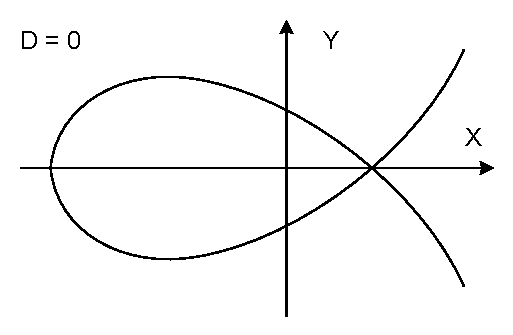
\includegraphics[height=2cm,keepaspectratio]{pic/elliptic-curve-2}}
	~~~~
	\subcaptionbox{$D<0$\label{fig:elliptic-curve-3}}{\includegraphics[height=2cm,keepaspectratio]{pic/elliptic-curve-3}}
	\caption{Эллиптические кривые с различными дискриминантами}
\end{figure}

\begin{enumerate}
    \item При $D>0$ график эллиптической кривой состоит из двух частей (см. рис.~\ref{fig:elliptic-curve-1}). Прямая, проходящая через точки $P(x_1; y_1)$ и $Q(x_2; y_2)$, обязательно пересечёт вторую часть кривой в точке с координатами $(x_3; \widetilde{y}_3)$, отображением которой является точка $R(x_3; y_3)$, где $y_3 = - \widetilde{y}_3$. Любые точки на кривой при $D>0$ являются элементами группы по сложению.
    \item Если $D=0$, то левая и правая части касаются в одной точке (см. рис.~\ref{fig:elliptic-curve-2}). Эти кривые называются сингулярными и не рассматриваются.
    \item Если $D<0$, то записанное выше уравнение~\ref{Wer} описывает одну кривую, представленную на рис.~\ref{fig:elliptic-curve-3}.
\end{enumerate}

Рассмотрим операцию сложения точек на эллиптической кривой при $D \ne 0$ (другие кривые не рассматриваются).

Пусть точки $P(x_1; y_1)$ и $Q(x_2; y_2)$ принадлежат эллиптической кривой (рис.~\ref{fig:elliptic-curve-1}). Определим операцию сложения точек
    \[ P + Q = R. \]

\begin{enumerate}
    \item Eсли $P \neq Q$, то точка $R$ определяется как отображение (инвертированная $y$-координата) точки, полученной пересечением эллиптической кривой и прямой $PQ$. Совместно решая уравнения кривой и прямой, можно найти координаты их точки пересечения. Зная координаты точки пересечения, можно вычислить и координаты искомой точки $R = (x_3; y_3)$, которые будут равны:
        \[ x_3 = \lambda^2 - x_1 - x_2, \]
        \[ y_3 = - y_1 + \lambda (x_1 - x_3), \]
где
        \[ \lambda = \frac{y_2 - y_1}{x_2 - x_1} \]
есть тангенс угла наклона между прямой, проходящей через точки $P$ и $Q$, и осью $x$.

	Теперь рассмотрим специальные случаи.
    \item Пусть точки совпадают: $P = Q$. Прямая $PQ$ превращается в касательную к кривой в точке $P$. Находим пересечение касательной с кривой, инвертируем $y$-координату полученной точки, это будет точка $P + P = R$. Тогда $\lambda$ -- тангенс угла между касательной, проведённой к эллиптической кривой в точке $P$, и осью $x$. Запишем уравнение касательной к эллиптической кривой в точке $(x; y)$ в виде:
            \[ 2 y y' = 3 x^2 + a. \]
        Производная равна
            \[ y' = \frac{3 x^2 + a}{2 y}, \]
        и
            \[ \lambda = \frac{3 x_1^2 + a}{2 y_1}. \]
        Координаты $R$ имеют прежний вид:
            \[ x_3 = \lambda^2 - x_1 - x_2, \]
            \[ y_3 = - y_1 + \lambda (x_1 - x_3), \]
    \item Пусть $P$ и $Q$ -- противоположные точки, то есть $P=(x; y)$ и $Q=(x; -y)$. Введём ещё одну точку на бесконечности и обозначим её $O$ (точка $O$ или точка 0 <<ноль>>, или альтернативное обозначение $\infty$). Результатом сложения двух противоположных точек определим точку $O$. Точка $Q$ в данном случае обозначается как $-P$:
        \[ P = (x; y), ~ -P = (x; -y), ~ P + (-P) = O. \]
    \item Пусть $P = (x; 0)$ лежит на оси $x$, тогда
        \[ -P = P, ~ P + P = O. \]
\end{enumerate}

Все точки эллиптической кривой, а также точка $O$ образуют коммутативную группу\index{группа!коммутативная} $\E(\R)$ относительно введённой операции сложения, то есть выполняются законы коммутативной группы:
\begin{itemize}
    \item сумма точек $P + Q$ лежит на эллиптической кривой;
    \item существует нулевой элемент -- это точка $O$ на бесконечности:
        \[ \forall P \in \E(\R): ~ O + P = P; \]
    \item для любой точки $P$ существует единственный обратный элемент $-P$:
        \[ P + (-P) = O; \]
    \item выполняется ассоциативный закон:
        \[ (P + Q) + F = P + (Q + F) = P + Q + F; \]
    \item выполняется коммутативный закон:
        \[ P + Q = Q + P. \]
\end{itemize}

Сложение точки с самой собой $d$ раз обозначим как умножение точки на число $d$:
    \[ \underbrace{P + P + \ldots + P}_{d \text{ раз}} = d P. \]


\subsection{Эллиптические кривые над конечным полем}

Эллиптические кривые можно строить не только над полем рациональных чисел, но и над другими полями. То есть координатами точек могут выступать не только числа, принадлежащие полю рациональных чисел $\R$, но и элементы поля комплексных чисел $\mathbb{C}$ или конечного поля $\F$. В криптографии нашли своё применение эллиптические кривые именно над конечными полями.

Далее будем рассматривать эллиптические кривые над конечным полем, являющимся кольцом вычетов по модулю нечётного простого\index{число!простое} числа $p$ (дискриминант не равен 0):
\begin{gather*}
    E: ~ y^2 = x^3 + a x + b, \\
    a, b, x, y \in \Z_p, \\
   \Z_p = \{0, 1, 2, \ldots, p-1\}.
\end{gather*}
Возможна также более компактная запись:
    \[ E: ~ y^2 = x^3 + a x + b \mod p.\]

Точкой эллиптической кривой является пара чисел
    \[ (x; y): x, y \in \Z_p, \]
удовлетворяющая уравнению эллиптической кривой, определённой над конечным полем $\Z_p$.

Операцию сложения двух точек $P = (x_1; y_1)$ и $Q = (x_2; y_2)$ определим точно так же, как и в случае кривой над полем вещественных чисел, описанном выше.

\begin{enumerate}
    \item Две точки $P = (x_1; y_1)$ и $Q = (x_2; y_2)$ эллиптической кривой, определённой над конечным полем $\Z_p$, складываются по правилу:
        \[
            P + Q = R \equiv (x_3; y_3),
        \] \[
            \begin{cases}
                x_3 = \lambda^2 - x_1 - x_2 \mod p,\\
                y_3 = - y_1 + \lambda (x_1 - x_3) \mod p,\\
            \end{cases}
        \]
        где
        \[
            \lambda = \begin{cases}
                \dfrac{y_2 - y_1}{x_2 - x_1} \mod p, & \text{ если } P \ne Q, \\
                \\
                \dfrac{3 x_1^2 + a}{2 y_1} \mod p, & \text{ если } P = Q. \\
            \end{cases}
        \]
    \item Сложение точки $P=(x; y)$ c противоположной \\
        $(-P) = (x; -y)$ даёт точку в бесконечности $O$:
        \begin{gather*}
          P + (-P) = O, \\
         (x_1; y_1) + (x_1; -y_1) = O, \\
         (x_1; 0) + (x_1; 0) = O. 
        \end{gather*}
\end{enumerate}

Мы рассматриваем эллиптические кривые над конечным полем $\Z_p$, где $p > 3$ -- простое\index{число!простое} число, элементы $\Z_p$ -- целые числа $\{0, 1, 2, \ldots, p-1\}$, то есть исследуем следующее уравнение двух переменных $x, y \in \Z_p$:
    \[ y^2 = x^3 + a x + b \mod p, \]
где $a, b \in \Z_p$ -- некоторые константы.

Как и в случае выше, множество точек над конечным полем $\Z_p$, удовлетворяющих уравнению эллиптической кривой, вместе с точкой в бесконечности $O$ образуют конечную группу $\E(\Z_p)$ относительно описанного закона сложения:\index{группа!точек эллиптической кривой}
    \[ \E(\Z_p) ~ \equiv~  O ~ \bigcup ~
        \left\{ (x; y) \in \Z_p \times \Z_p ~\Big|~ y^2 = x^3 + a x + b \mod p \right\}. \]

По теореме Хассе\index{теорема!Хассе} порядок группы точек $|\E(\Z_p)|$ оценивается как
    \[ (\sqrt{p}-1)^2 \leq |\E(\Z_p)| \leq (\sqrt{p}+1)^2, \]
или, в другой записи,
    \[ \Big| |\E(\Z_p)| - p - 1 \Big| \leq 2 \sqrt{p}. \]

\subsection{Примеры группы точек}

\subsubsection{Пример 1}

Пусть эллиптическая кривая задана уравнением
    \[ E: ~ y^2 = x^3 + 1 \mod 7. \]
Найдём все решения этого уравнения, а также количество точек $|\E(\Z_p)|$ на этой эллиптической кривой. Для нахождения решений уравнения составим следующую таблицу:

\begin{center} \begin{tabular}{|c|c|c|c|c|c|c|c|}
    \hline
    $x$ & 0 & 1 & 2 & 3 & 4 & 5 & 6 \\
    \hline
    $y^2$ & 1 & 2 & 2 & 0 & 2 & 0 & 0 \\
    \hline
    $y_1$ & 1 & 3 & 3 & 0 & 3 & 0 & 0 \\
    \hline
    $y_2 = - y_1 \mod p$ & 6 & 4 & 4 &   & 4 &   &   \\
    \hline
\end{tabular} \end{center}

Выпишем все точки, принадлежащие данной эллиптической кривой $\E(\Z_p)$:
\[
    \begin{array}{cccc}
        P_1 = O, & P_2 = (0; 1), & P_3 = (0; 6), & P_4 = (1; 3), \\
        P_5 = (1; 4), & P_6 = (2; 3), & P_7 = (2; 4), & P_8 = (3; 0), \\
        P_9 = (4; 3), & P_{10} = (4; 4), & P_{11} = (5; 0), & P_{12} = (6; 0). \\
    \end{array}
\]

Получили
    \[ |\E(\Z_p)| = 12. \]

Проверим выполнение неравенства Хассе:
    \[ \left| 12 - 7 - 1 \right| = 4 < 2 \sqrt{7}. \]
Следовательно, неравенство Хассе выполняется.

Минимальное натуральное число $s$ такое, что
\[ \underbrace{P + P + \ldots + P}_{s} \equiv s P = O, \]
будем называть \emph{порядком точки $P$}.

%Теорема Лагранжа определяет порядок подгруппы.

\subsubsection{Пример 2}

Группа точек эллиптической кривой
    \[ y^2 = x^3 + 5 x + 6 \mod 17 \]
состоит из точек:
\[ \begin{array}{ccccccc}
    \E(\Z_p) & =~ \Big\{ & (-8; \pm 7), & (-7; \pm 6), & (-6; \pm 7), &   & \\
             &           & (-5; \pm 3), & (-3; \pm 7), & (-1; 0),     & O & \Big\}. \\
\end{array} \]

Порядок группы:
    \[ |\E(\Z_p)| = 12. \]

Порядок группы точек по теореме Хассе:
    \[ (\sqrt{p}-1)^2 \leq |\E(\Z_p)| \leq (\sqrt{p}+1)^2, \]
    \[ 10 \leq 12 \leq 26. \]

Порядки возможных подгрупп: 2, 3, 4, 6 (все возможные делители порядка группы 12).

Найдём порядок точки $A = (-8; 7)$. Так как возможные порядки подгрупп (и всех точек группы) известны, нужно проверить только их.

\begin{itemize}
\item $2A = A + A = (-5; 3)$:
\[\begin{aligned}
& R = P + P, P = (-8; 7), \\
& \lambda = \frac{3 x_P^2 + a}{2y_P} = \frac{3 \cdot (-8)^2 + 5}{2 \cdot 7} = 8 \mod 17, \\
& x_R = \lambda^2 - 2x_P = 8^2 - 2 \cdot (-8) = -5 \mod 17, \\
& y_R = \lambda (x_P - x_R) - y_P = 8 \cdot ((-8) - (-5)) - 7 = 3 \mod 17, \\
& R = (-5; 3). \\
\end{aligned}\]

\item $3A = 2A + A = (-6; 7)$:
\[\begin{aligned}
& R = P + Q, P = (-8; 7), Q = (-5; 3), \\
& \lambda = \frac{y_Q - y_P}{x_Q - x_P} = \frac{3 - 7}{-5 - (-8)} = -7 \mod 17, \\
& x_R = \lambda^2 - x_P - x_Q = (-7)^2 - (-8) - (-5) = -6 \mod 17, \\
& y_R = \lambda (x_P - x_R) - y_P = -7 \cdot (-8 - (-6)) - 7 = 7 \mod 17, \\
& R = (-6; 7). \\
\end{aligned}\]

\item $4A = 2A + 2A = (-5; 3) + (-5; 3) = (-3; 7)$.

\item $6A = 3A + 3A = (-6; 7) + (-6; 7) = (-1; 0)$.

\item $12A = 6A + 6A = (-1; 0) + (-1; 0) = 0$.

\end{itemize}

Найденный порядок точки $A = (-8; 7)$ равен 12, следовательно, она является генератором всей группы.

В таблице~\ref{tab:elliptic-group-sample} найдены порядки точек и циклические подгруппы группы точек $\E(\Z_p)$ такой же эллиптической кривой
    \[ y^2 = x^3 + 5 x + 6 \mod 17. \]
Группа циклическая, число генераторов:
    \[ \varphi(12) = 4. \]
Циклические подгруппы:
    \[ \Gr^{(2)}, ~ \Gr^{(3)}, ~ \Gr^{(4)}, ~ \Gr^{(6)}, \]
верхний индекс обозначает порядок подгруппы.

\begin{table}[!ht]
    \centering
    \caption{Генераторы и циклические подгруппы группы точек эллиптической кривой\label{tab:elliptic-group-sample}}
    \resizebox{\textwidth}{!}{
    \begin{tabular}{|c|l|c|}
        \hline
        Элемент & Порождаемая группа или подгруппа & Порядок \\
        \hline
        $(-8; \pm 7) $ & Вся группа $\E(\Z_p)$ & 12, генератор \\
        $(-7; \pm 6) $ & Вся группа $\E(\Z_p)$ & 12, генератор \\
        $(-6; \pm 7) $ & $\Gr^{(4)} ~=~ \left\{ ~ (-6; \pm 7), ~ (-1; 0), ~ O ~ \right\}$ & 4 \\
        $(-5; \pm 3) $ & $\Gr^{(6)} ~=~ \left\{ ~ (-5; \pm 3), ~ (-3; \pm 7), ~ (-1; 0), ~ O ~ \right\}$ & 6 \\
        $(-3; \pm 7) $ & $\Gr^{(3)} ~=~ \left\{ ~ (-3; \pm 7), ~ O ~ \right\}$ & 3\\
        $(-1; 0)     $ & $\Gr^{(2)} ~=~ \left\{ ~ (-1; 0), ~ O ~ \right\}$ & 2\\
        \hline
    \end{tabular}
    }
\end{table}

\subsection{Эллиптические кривые в скрученной форме Эдвардса}\label{sec:twisted-edward-curves}

Любую эллиптическую кривую с помощью замены координат можно представить в рассмотренной ранее форме Вейерштрасса. Используя данное представление мы ранее ввели операцию сложения точек, умножения точки на число, смогли описать группу точек и циклическую подгруппу. Однако в отдельных случаях эллиптические кривые можно записать в другой, более удобной для частных задач форме. Например, любые эллиптические кривые над алгебраически замкнутым полем можно задать с помощью следующего уравнения:

\[ \begin{array}{l}
	ax^2+y^2=1+dx^2y^2.
\end{array} \]

Примеры кривых, заданных этим уравнениям при различных значениях $d$, приведены на рис.~\ref{pic:Edward-curves}. Данное кривые в указанном представлении называются эллиптическими кривыми в скрученной форме Эдвардса (\langen{Twisted Edwards Curves}, \cite{Bernstein:Birkner:Joye:Lange:Peters:2008}).

\begin{figure}
	\centering
	\includegraphics[width=0.5\textwidth]{pic/Edward-curves}
	\caption{Эллиптические кривые в скрученной форме Эдвардса при значениях (от внешней фигуры ко внутренней) $d = +0{,}9, -\sqrt{8}, -300$}
	\label{pic:Edward-curves}
\end{figure}

Для данной формы формулы сложения точек задаются одним и тем же способом для любых случаев. В этом важное отличие от формы Вейерштрасса, для которой есть частный случай сложения точки самой с собой (с отдельной формулой вычисления угла наклона касательной). Формулы сложения выглядят так:

\[ \begin{array}{ll}
	P + Q = R \equiv (x_3; y_3), \\
	
	\begin{cases}
		x_3 = \frac{x_1 y_2 + x_2 y_1}{ 1 + dx_1x_2y_1y_2},\\
		y_3 = \frac{ y_1 y_2 - x_1 x_2 }{1 - d x_1 x_2 y_1 y_2}.\\
	\end{cases}

\end{array} \]

При переходе к построению кривых над конечным полем, оказывается, что не все кривые, представимые в форме Вейерштрасса, могут быть представлены в скрученной форме Эдвардса. Для этого необходимо, чтобы порядок кривой $\|E\|$ делился на $4$. Однако если такие кривые использовать для криптографических целей, это даёт значимые преимущества:

\begin{itemize}
	\item меньшая трудоёмкость операций сложения точек;
	\item отсутствие частных случаев для формул сложения (усложнение атак по сторонним каналам с различением времени);
\end{itemize}

\subsection{Конвертация из скрученной формы Эдвардса в форму Вейерштрасса}

Кривая в скрученной форме Эдвардса:
\[eu^2+v^2=1+du^2v^2 \mod p.\]\\

Кривая в форме Вейерштрасса:\\
\[ y^{2} = x^{3} + ax + b \mod p.\]

Зная коэффициенты $d$ и $e$ кривой в скрученной форме Эдвардса можно найти коэффициенты $a$ и $b$ эквивалентной кривой в форме Вейерштрасса:

\[ \begin{array}{l}
	s = (e - d)/4, \\
    t = (e + d)/6, \\
	a = s^2 - 3t^2, \\
	b = 2t^3 - ts^2. \\
\end{array} \]

И определить правила преобразования координат $(u, v)$ и $(x, y)$ между двумя кривыми:

\[ \begin{array}{l}
(u,v) \longrightarrow(x, y)= (\frac{s(1+v)}{1-v}+t,\frac{s(1+v)}{(1-v)u}), \\
(x,y) \longrightarrow(u, v)= (\frac{x-t}{y}, \frac{x-t-s}{x-t+s}). \\
\end{array} \]

Нахождение коэффициентов для кривой в скрученной форме Эдвардса по эквивалентной в форме Вейерштрасса является более сложной и нетривиальной задачей, включающей нахождение корней кубического уравнения $x^{3} + ax + b = 0 \mod p$. Кроме того, как было сказано ранее, не все кривые в форме Вейерштрасса имеют эквивалентную кривую в скрученной форме Эдвардса.

\subsection{Пример группы точек кривой в скрученной форме Эдвардса}

Кривая $x^2+y^2=1+6x^2y^2 \mod 11$.

Все точки кривой:

\[ \begin{array}{lll}
(0; 1), & (2; 5), & (5; 2), \\
(1; 0), & (5; 9), & (2; 6), \\
(0; 10), & (9; 5), & (6; 9), \\
(10; 0), & (6; 2), & (9; 5). \\
\end{array} \]

Нейтральным элементом является точка $(0; 1)$. 

Данная группа точек является циклической группой, её генератором выступает точка $(2; 5)$ (рис.~\ref{pic:Twisted-Edwards-Curve-Example}):

\[ \begin{array}{lllllll}
(2; 5) & \to (6; 9) & \to (10; 0) & \to (6; 2) & \to (2; 6) & \to (0; 10) & \to \\
       & \to (9; 6) & \to (5; 2)  & \to (1; 0) & \to (5; 9) & \to (9; 5)  & \to (0; 1).
\end{array} \]

\begin{figure}
	\centering
	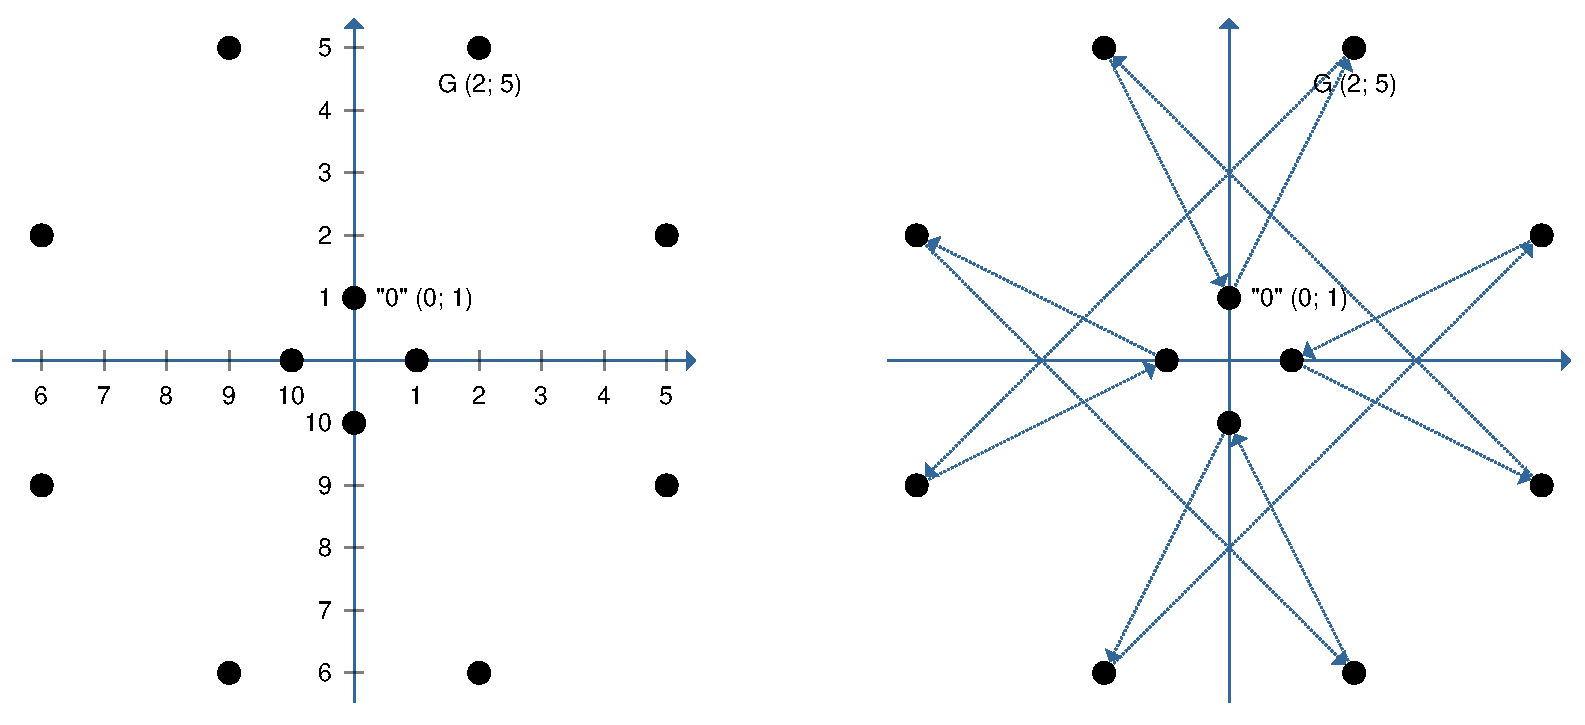
\includegraphics[width=1\textwidth]{pic/Twisted-Edwards-Curve-Example}
	\caption{Группа точек эллиптической кривой в скрученной форме Эдвардса $x^2+y^2=1+6x^2y^2 \mod 11$}
	\label{pic:Twisted-Edwards-Curve-Example}
\end{figure}

Данная группа изоморфна группе вычетов по сложению $\Z_{12}$. Можно удостовериться, что сложение двух точек $P (6; 9)$ и $Q(10; 0)$ будет соответствовать результату сложения элементов <<2>> и <<3>> в группе $\Z_{12}$:

\[ \begin{array}{l}
	R = P (6; 9) + Q (10; 0), \\
	x_R = \frac{x_1 y_2 + x_2 y_1}{1 + d x_1 x_2 y_1 y_2} = \frac{6 \times 0 + 10 \times 9}{1 + 6 \times 6 \times 10 \times 9 \times 0} = \frac{90}{1} = 2 \mod 11, \\
	y_R = \frac{y_1 y_2 - x_1 x_2}{1 - d x_1 x_2 y_1 y_2} = \frac{9 \times 0 - 6 \times 10}{1 - 6 \times 6 \times 10 \times 9 \times 0} = \frac{-60}{1} = 6 \mod 11, \\
	R (2; 6) \equiv \text{<<5>>}.
\end{array} \]

Группа не имеет эквивалентной группы точек эллиптической кривой в форме Вейерштрасса над конечным полем $\F_{11}$. Группа точек соответствующей кривой $y^2 = x^3 + 6 \bmod 11$ имеет только 11 элементов в группе.

\index{группа!точек эллиптической кривой|)}

\section{Классы сложности задач}

Данный раздел поясняет обоснованность стойкости криптосистем с открытым ключом и имеет лишь косвенное отношение к дискретной математике.

Машина Тьюринга (МТ) (модель, представляющая любой вычислительный алгоритм) состоит из следующих частей:
\begin{itemize}
    \item неограниченная лента, разделённая на клетки; в каждой клетке содержится символ из конечного алфавита, содержащего пустой символ blank; если символ ранее не был записан на ленту, то он считается blank;
    \item печатающая головка, которая может считать, записать символ $a_i$ и передвинуть ленту на 1 клетку влево или вправо $d_k$;
    \item конечная таблица действий
    \[ (q_i, a_j) \rightarrow (q_{i1}, a_{j1}, d_k), \]
где $q$ -- состояние машины.
\end{itemize}

Если таблица переходов однозначна, то машина Тьюринга\index{машина Тьюринга} называется детерминированной. \emph{Детерминированная} машина Тьюринга может \emph{имитировать} любую существующую детерминированную ЭВМ. Если таблица переходов неоднозначна, то есть $(q_i, a_j)$ может переходить по нескольким правилам, то машина \emph{недетерминированная}.

Класс задач $\set{P}$ -- задачи, которые могут быть решены за \emph{полиномиальное} время\index{задача!полиномиальная} на \emph{детерминированной} машине Тьюринга. Пример полиномиальной сложности (количество битовых операций)
    \[ O(k^{\textrm{const}}), \]
где $k$ -- длина входных параметров алгоритма. Операция возведения в степень в модульной арифметике $a^b \mod n$ имеет кубическую сложность $O(k^3)$, где $k$ -- двоичная длина чисел $a,b,n$.

Класс задач $\set{NP}$ -- обобщение класса $\set{P} \subseteq \set{NP}$, включает задачи, которые могут быть решены за \emph{полиномиальное} время на \emph{недетерминированной} машине Тьюринга. Пример сложности задач из $\set{NP}$ -- экспоненциальная сложность\index{задача!экспоненциальная}
    \[ O(\textrm{const}^k). \]
Алгоритм Гельфонда решения задачи дискретного логарифмирования (нахождения $x$ для заданных основания $g$, модуля $p$ и $a = g^x \mod p$), описанный в разделе криптостойкости системы Эль-Гамаля\index{криптосистема!Эль-Гамаля}, имеет сложность $O(e^{k/2})$, где $k$ -- двоичная длина чисел.

В криптографии полиномиальные задачи (относящиеся к классу $\set{P}$) считаются \emph{лёгкими и вычислимыми} на ЭВМ, которые являются детерминированными машинами Тьюринга. Для них, по определению, существуют алгоритмы, работающие за время, полиномиальное относительно размера входных данных. Задачи, относящиеся к классу $\set{NP}$, считаются \emph{трудными и невычислимыми} на ЭВМ, так как все известные на сегодняшний день алгоритмы решения таких задач (в общем случае) требуют экспоненциального времени, а значит всегда можно выбрать такой размер входных данных (читай -- размер ключа шифрования), что время вычисления станет сравнимым с возрастом Вселенной.

Класс $\set{NP}$-полных задач -- подмножество задач из $\set{NP}$, для которых не известен полиномиальный алгоритм для детерминированной машины Тьюринга, и все задачи могут быть сведены друг к другу за полиномиальное время на \emph{детерминированной} машине Тьюринга. Например, задача об укладке рюкзака является $\set{NP}$-полной.

Стойкость криптосистем с \emph{открытым} ключом, как правило, основана на $\set{NP}$ или $\set{NP}$-полных задачах:
\begin{enumerate}
    \item RSA\index{криптосистема!RSA} -- $\set{NP}$-задача факторизации (строго говоря, основана на трудности извлечения корня степени $e$ по модулю $n$).
    \item Криптосистемы типа Эль-Гамаля\index{криптосистема!Эль-Гамаля} -- $\set{NP}$-задача дискретного логарифмирования.
\end{enumerate}

\emph{Нерешённой} проблемой является доказательство неравенства
    \[ \set{P} \neq \set{NP}. \]
Именно на гипотезе о том, что для некоторых задач не существует полиномиальных алгоритмов, и основана стойкость криптосистем с открытым ключом.

\section{Метод индекса совпадений}
\selectlanguage{russian}
\label{chap:coincide-index}

Приведём теоретическое обоснование метода индекса совпадений. Пусть алфавит имеет размер $A$. Перенумеруем его буквы числами от $1$ до $A$. Пусть заданы вероятности появления каждой буквы
    \[ \mathcal{P} = \left\{ {p_1 ,p_2 ,  \ldots , p_A } \right\}. \]
В простейшей модели языка предполагается, что тексты состоят из последовательности букв, порождаемых источником независимо друг от друга с известным распределением $\mathcal{P}$.

Найдём индекс совпадений для различных предположений относительно распределений букв последовательности. Сначала рассмотрим случай, когда вероятности всех букв одинаковы. Пусть
    \[ \mathbf{X} = \left[ X_1, X_2, \dots, X_L \right] \]
случайный текст с распределением
    \[ \mathcal{P}_1 = \left\{ p_{11}, p_{12}, \dots, p_{1A} \right\}. \]
Найдём индекс совпадений
    \[ I_c(\mathcal{P}_1), \]
то есть вероятность того, что в случайно выбранной паре позиций находятся одинаковые буквы.

Для пары позиций $(k,j)$ найдём условную вероятность $P \left( X_k  = X_j \mid (k,j) \right)$:
    \[ P \left( X_k  = X_j \mid (k,j) \right) ~=~ \sum\limits_{i=1}^A p_{1i}^2 ~\equiv~ k_{p_1}. \]
Эта вероятность не зависит от выбора пары позиций $(k,j)$.

Так как число различных пар равно $\frac{L(L - 1)}{2}$, то вероятность случайного выбора пары $(k,j)$ равна
    \[ P_{(K,J)} (k,j) = \frac{2}{L(L - 1)}. \]
Следовательно,
\[
    I(\mathcal{P}_1) ~= \sum \limits_{1 \leq k < j \leq L} P_{(K,J)}(k,j) ~\cdot~ P(X_k  = X_j \mid (k,j)) =
\] \[
    = \sum \limits_{1 \leq k < j \leq L} \frac{2}{L(L - 1)} k_{p_1} = k_{p_1}.
\]

Найдём теперь аналогичную вероятность $I\left( {\mathcal{P}_1 ,\mathcal{P}_2 } \right)$ для случая, когда последовательность независимых случайных букв может быть представлена в виде
\[
\mathbf{X} = \left[ {\begin{array}{*{20}c}
   {X_1 ,}  \\
   {Y_1 ,}  \\
 \end{array} \begin{array}{*{20}c}
   {X_2 ,}  \\
   {Y_2 ,}  \\
 \end{array} \begin{array}{*{20}c}
   { \ldots ,}  \\
   { \ldots ,}  \\
 \end{array} \begin{array}{*{20}c}
   {X_{L/2} }  \\
   {Y_{L/2} }  \\
 \end{array} } \right],
\]
где одинаково распределенные случайные буквы в первой строке имеют распределение
    \[ \mathcal{P}_1  = \left\{ {p_{11} ,p_{12} ,  \ldots , p_{1A} } \right\}, \]
а одинаково распределенные случайные буквы во второй строке имеют другое распределение
    \[ \mathcal{P}_2  = \left\{ {p_{21} ,p_{22} ,  \ldots , p_{2A} } \right\}. \]
В этом случае сумму по всем парам мы разделяем на три суммы: по парам внутри позиций первой строки, по парам внутри позиций второй строки и по парам, в которых первая позиция берётся из первой строки, а вторая -- из второй:
{ \small
\[
    I(\mathcal{P}_1, \mathcal{P}_2) =
        \frac{2}{L(L - 1)} \cdot \left(
        \sum \limits_{1 \leq k < j \leq L/2} P( X_k  = X_j \mid ( k,j )) ~~ + \right.
\] \[
        \left. + \sum\limits_{1 \leq k < j \leq L/2} P(Y_k  = Y_j \mid (k,j)) ~~+~~
            \sum\limits_{k=1}^{L/2} \sum\limits_{j=1}^{L/2} {P(X_k = Y_j \mid (k,j))} \right) =
\] \[
    = \frac{2}{L(L - 1)} \left( \frac{1}{2} \frac{L}{2} \left( \frac{L}{2} - 1 \right) k_{p_1} +
        \frac{1}{2} \frac{L}{2} \left( \frac{L}{2} - 1 \right) k_{p_2} +
        \left( \frac{L}{2} \right)^2 \sum \limits_{i = 1}^A p_{1,i} p_{2,i} \right) =
\] \[
    = \frac{2}{L(L - 1)} \left( \frac{1}{2} \frac{L}{2} \left( \frac{L}{2} - 1 \right) k_{p_1} +
        \frac{1}{2} \frac{L}{2} \left( \frac{L}{2} - 1 \right) k_{p_2} +
        \left( \frac{L}{2} \right)^2 k_{p_1, p_2} \right),
\] }
где обозначено
    \[ k_{p_1, p_2}  = \sum\limits_{i=1}^A p_{1,i} p_{2,i}. \]


В общем случае рассмотрим последовательность, представленную в виде матрицы, состоящей из $m$ строк и $\frac{L}{m}$ столбцов, где
\[
{\mathbf X} = \left[ {\begin{array}{*{20}c}
   {X_1 } & {X_2 } &  \ldots  & {X_{L/m} }  \\
   {Y_1 } & {Y_2 } &  \ldots  & {Y_{L/m} }  \\
    \vdots  &  \vdots  &  \vdots  &  \vdots   \\
   {Z_1 } & {Z_2 } &  \ldots  & {Z_{L/m} }  \\
\end{array}} \right].
\]
Считаем, что одинаково распределенные случайные буквы в первой строке имеют распределение
    \[ P_1  = \left\{ {p_{11} ,p_{12} ,  \ldots , p_{1A} } \right\}, \]
одинаково распределённые случайные буквы во второй строке имеют распределение
    \[ P_2  = \left\{ {p_{21} ,p_{22} ,  \ldots , p_{2A} } \right\} \]
и т.~д., одинаково распределенные случайные буквы $m$-й строки имеют распределение
    \[ P_m  = \left\{ {p_{m1},p_{m2} ,  \ldots , p_{mA} } \right\}. \]

Для вычисления вероятности того, что в случайно выбранной паре позиций будут одинаковые буквы, выполним суммирование по различным парам внутри строк и по парам между различными строками. Аналогично предыдущему случаю получим
{ \small
\[
    I(\mathcal{P}_1, \mathcal{P}_2, \ldots, \mathcal{P}_m ) ~=
\] \[
    =~ \frac{2}{L(L - 1)} \left( \frac{1}{2} \frac{L}{m} \left( \frac{L}{m} - 1 \right) k_{p_1} ~+~
        \frac{1}{2} \frac{L}{m} \left( \frac{L}{m} - 1 \right) k_{p_2} ~+ \right.
\] \[
        +~ \dots ~+~ \left. \frac{1}{2} \frac{L}{m} \left( \frac{L}{m} - 1 \right) k_{p_m} \right) ~+
\] \[
       +~ \frac{2}{L(L - 1)} \left( \left( \frac{L}{m} \right)^2 k_{p_1, p_2} +
         \left( \frac{L}{m} \right)^2 k_{p_1, p_3} + \dots +
        \left( \frac{L}{m} \right)^2 k_{p_{m - 1}, p_m } \right).
\] }
Первая сумма содержит $m$ слагаемых, вторая -- $ \frac{m(m-1)}{2}$ слагаемых. Полагая
    \[ k_{p_1} = k_{p_2} = \dots = k_{p_m} = k_p, \]
    \[ k_{p_i p_j } = k_r = \frac{1}{A}, ~ i \ne j, \]
получим после несложных выкладок
    \[ m = \frac{k_p  - k_r}{I - k_r  + \frac{k_p  - I}{L}}. \]


\chapter{Примеры задач}
\selectlanguage{russian}
\taskinit

В данном разделе приведены примеры задач, которые использовались на контрольных работах в МФТИ по курсу <<Защита информации>> в 2011--2015 годах.

\section{Математические основы}
\tasksection

\tasknumber Найдите общее количество и перечислите генераторы аддитивной циклической группы $\mathbb{Z}_{33}$ с операцией в виде сложения чисел по модулю 33.
\medbreak
\textbf{Ответ:} 20: [1, 2, 4, 5, 7, 8, 10, 13, 14, 16, 17, 19, 20, 23, 25, 26, 28, 29, 31, 32].
\bigbreak

\tasknumber Вычислить в поле Галуа $GF\left( {2^{5} } \right)$, $m\left( x \right) = x^{5} + x^{3} + x^{2} + x + 1$, следующее значение: $28 \times 29 + 23^2$. Многочлены заданы как десятичное представление двоичных коэффициентов, свободный член многочлена соответствует младшему биту двоичного представления. В ответе привести в десятичном представлении результаты умножения, возведения в степень и сложения.
\medbreak
\textbf{Решение:}
\begin{itemize}\itemsep1pt \parskip0pt \parsep0pt
	\item $a = "28" \Rightarrow a\left( x \right) = x^{4} + x^{3} + x^{2}$;
	\item $b = "29" \Rightarrow b\left( x \right) = x^{4} + x^{3} + x^{2} + 1$;
	\item $c = "23" \Rightarrow c\left( x \right) = x^{4} + x^{2} + x + 1$;
	\item $a \left( x \right) \times b \left( x \right) = x^{4} + x^{3} + x + 1 \Rightarrow a \times b = "27"$;
	\item $c \left( x \right)^2 = x^{4} + x^{3} + x^{2} \Rightarrow c^2 = "28"$;
	\item $result\left( x \right) = x^{2} + x + 1 \Rightarrow result = "7"$.
\end{itemize}
\medbreak
\textbf{Ответ:} <<27>>; <<28>>; <<7>>.
\bigbreak

\tasknumber Вычислить в поле Галуа $GF\left( 27 \right)$, $m\left( x \right) = x^{3} + x^{2} + x + 2$, следующее значение: $26 \times 11 + 25^2$. Многочлены заданы как десятичное представление троичных коэффициентов, свободный член многочлена соответствует младшему биту троичного представления. В ответе привести в десятичном представлении результаты умножения, возведения в степень и сложения.
\medbreak
\textbf{Решение:}
\begin{itemize}\itemsep1pt \parskip0pt \parsep0pt
	\item $a = "26" \Rightarrow a\left( x \right) = 2 x^{2} + 2 x + 2$;
	\item $b = "11" \Rightarrow b\left( x \right) = x^{2} + 2$;
	\item $c = "25" \Rightarrow c\left( x \right) = 2 x^{2} + 2 x + 1$;
	\item $a \left( x \right) \times b \left( x \right) = x^{2} + 1 \Rightarrow a \times b = "10"$;
	\item $c \left( x \right)^2 = x + 2 \Rightarrow c^2 = "5"$;
	\item $result\left( x \right) = x^{2} + x \Rightarrow result = "12"$.
\end{itemize}
\medbreak
\textbf{Ответ:} <<10>>; <<5>>; <<12>>.
\bigbreak

\tasknumber Используя алгоритм быстрого возведения в степень (с помощью разложения показателя степени по степеням двойки по схеме <<слева направо>>), вычислить ${175}^{235} \mod {257}$.
\medbreak
\textbf{Решение:}
\begin{itemize}\itemsep1pt \parskip0pt \parsep0pt
	\item двоичная форма записи степени: $235_{10} = 11101011_{2}$;
	\item полное выражение для вычисления: $(((((((1 \times {175}^1)^2 \times {175}^1)^2 \times {175}^1)^2 \times {175}^0)^2 \times {175}^1)^2 \times {175}^0)^2 \times {175}^1)^2 \times {175}^1\mod 257$;
	\item шаг \No1: $1^2 \times 175 \mod 257  = 175$;
	\item шаг \No2: $175^2 \times 175 \mod 257 = 154$;
	\item шаг \No3: $154^2 \times 175 \mod 257 = 7$;
	\item шаг \No4: $7^2 \mod 257 = 49 \mod 257 = 49$;
	\item шаг \No5: $49^2 \times 175 \mod 257 = 237$;
	\item шаг \No6: $237^2 \mod 257 = 143$;
	\item шаг \No7: $143^2 \times 175 \mod 257 = 107$;
	\item шаг \No8: $107^2 \times 175 \mod 257 = 3$.
\end{itemize}
\medbreak
\textbf{Ответ:} 3.
\bigbreak

\section{Общие определения и теория}
\tasksection

\tasknumber Рассмотрим множество паролей, состоящих из 12 строчных и заглавных латинских букв, а также цифр.
\begin{itemize}\itemsep1pt \parskip0pt \parsep0pt
\item Каков размер этого множества?
\item Сколько времени потребуется на взлом шифротекста, зашифрованного данным паролем, если предположить, что во взломе участвуют все компьютеры мира (7~млрд.), а средний компьютер перебирает 30~000 паролей в секунду?\footnote{См. скорости перебора MD5-хэшей\index{хэш-функция!MD5} на странице \texttt{http://openwall.info\hspace{0pt}/wiki\hspace{0pt}/john\hspace{0pt}/benchmarks}}
\item Каковы затраты электроэнергии в денежном эквиваленте, если средний компьютер потребляет мощность 400~Вт, а стоимость 1~кВт$\times$час составляет 4,68~рубля?
\end{itemize}
\medbreak
\textbf{Решение:}
\begin{itemize}\itemsep1pt \parskip0pt \parsep0pt
	\item общее количество символов: $26 + 26 + 10 = 62$;
	\item общее количество паролей: $62^{12} \approx 3{,}226\times 10^{21}$;
	\item время на перебор: $62^{12} / (3 \times 10^5) / (7 \times 10^9 ) \approx 1{,}54 \times 10^{6}$ сек.;
	\begin{itemize}\itemsep1pt \parskip0pt \parsep0pt
		\item в минутах: $\approx 25605$;
		\item в часах: $\approx 427$;
		\item в днях: $\approx 18$;
	\end{itemize}
	\item стоимость: $427 \times (7 \times 10^9 ) \times 0{,}4 \times 4{,}68 \approx 5{,}59 \times 10^{12}$ руб.
\end{itemize}
\medbreak
\textbf{Ответ:} паролей $3{,}226 \times 10^{21}$; на перебор нужно $1{,}54 \times 10^6$ секунд ($\approx 18$ дней); затраты -- 5,6 триллиона рублей.
\bigbreak

\tasknumber Источник открытого текста характеризуется случайной величиной $X$, принимающей два значения $x_1$ и $x_2$ с вероятностями $p \left( x = x_1 \right) = 1/5$ и $p \left( x = x_2 \right) = 4/5$ соответственно. Источник ключей характеризуется случайной величиной $Z$, независимой от величины $X$, принимающей два значения $z_1$ и $z_2$ с вероятностями $p \left( z = z_1 \right) = 1/6$ и $p \left( z = z_2 \right) = 5/6$ соответственно. Функция шифрования $E_{z} \left( x \right)$ задаётся следующими правилами: $\left( x_1, z_1 \right) \to y_1$, $\left( x_1, z_2 \right) \to y_2$, $\left( x_2, z_1 \right) \to y_2$, $\left( x_2, z_2 \right) \to y_1$.
\begin{enumerate}\itemsep1pt \parskip0pt \parsep0pt
	\item Найдите собственную информацию каждого из сообщений открытого текста в битах.
	\item Найдите энтропию источника сообщений, источника ключей и шифротекста в битах.
	\item Найдите взаимную информацию открытого текста и ключа в битах.
	\item Найдите взаимную информацию открытого текста и шифротекста в битах.
	\item Найдите взаимную информацию ключа и шифротекста в битах.
	\item Найдите апостериорное распределение вероятностей открытого текста для обоих вариантов перехваченных злоумышленником шифротекстов $y_1$ и $y_2$. Используя вычисленные значения, определите, является ли данная шифросистема абсолютно надёжной. Если нет, то что в данной криптосистеме необходимо поменять? Покажите, что апостериорные вероятности после доработки будут удовлетворять необходимым требованиям абсолютно надёжной криптосистемы.
\end{enumerate}
\medbreak
\textbf{Ответ:}
\begin{itemize}\itemsep1pt \parskip0pt \parsep0pt
	\item $I \left( x_1 \right) = \log_2 5 = 2{,}322$ бит; $I \left( x_2 \right) = \log_2 5/4 = 0{,}322$ бит;
	\item $H \left( X \right) = 0{,}722$ бит; $H \left( Z \right) = 0{,}650$ бит; $H \left( Y \right) = 0{,}881$ бит;
	\item $I \left( X ; Z \right) = 0$ бит; $I \left( X; Y \right) = 0{,}231$ бит; $I \left( Y; Z \right) = 0{,}159$ бит;
	\item $p \left( x_1 | y_1 \right) = 1/21$; $p \left( x_2 | y_1 \right) = 20/21$; $p \left( x_1 | y_2 \right) = 5/9$; $p \left( x_2 | y_2 \right) = 4/9$; не является.
\end{itemize}

\section{КСГПСЧ и потоковые шифры}
\tasksection

\tasknumber Привести следующие два элемента последовательности, сформированной линейным конгруэнтным методом, если предыдущие 3 элемента последовательности такие: 348, 65, 139, а все вычисления выполняются в поле $\mathbb{F}_{499}$.
\medbreak
\textbf{Решение:}
\begin{itemize}\itemsep1pt \parskip0pt \parsep0pt
	\item используя предыдущие значения выхода генератора, строим систему уравнений:
		\[\left\{ {\begin{array}{*{20}c}
		348 \cdot a + c = 65 \mod 499 \\
		65 \cdot a + c = 139 \mod 499 \\
		\end{array} } \right. ;\]
	\item из системы уравнений находим $a = 467$ и $c = 223$;
	\item используя найденные значения, находим следующие элементы последовательности;
	\begin{itemize}\itemsep1pt \parskip0pt \parsep0pt
		\item $x_{3} = a x_{2} + c \mod m = 467 \cdot 139 + 223 \mod 499 = 266$;
		\item $x_{4} = a x_{3} + c \mod m = 467 \cdot 266 + 223 \mod 499 = 194$.
	\end{itemize}
\end{itemize}
\medbreak
\textbf{Ответ:} 266, 194.
\bigbreak

\tasknumber Приведите \emph{предыдущие} 5 бит выхода генератора псевдослучайной последовательности, основанного на регистре сдвига с линейной обратной связью, если известно, что характеристический полином регистра — $m\left(x\right)=x^{5} + x^{3} + 1$ (см. рис.), а дальнейшая последовательность такова: $1, 1, 0, 1, 0, 1$.
\begin{center}
	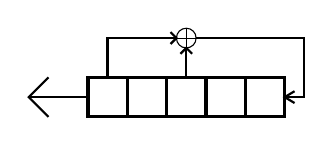
\begin{tikzpicture}[scale=0.05]
		\draw[black,very thick] (30,30) -- (30,40) -- (40,40) -- (40,30) -- (30,30) -- (30,40);
		\draw[black,thick] (35,40) -- (35,50) -- (35,50) -- (37.5,50);
		\draw[black,very thick] (40,30) -- (40,40) -- (50,40) -- (50,30) -- (40,30) -- (40,40);
		\draw[black,very thick] (50,30) -- (50,40) -- (60,40) -- (60,30) -- (50,30) -- (50,40);
		\draw[black,thick] (55,40) -- (55,47.5);
		\draw[black,thick] (53.5,46) -- (55,47.5) -- (56.5,46);
		\draw[black,thick] (37.5,50) -- (52.5,50);
		\draw[black,thick] (51,51.5) -- (52.5,50) -- (51,48.5);
		\draw (55,50) circle [radius=2.5];
		\draw[black] (52.5,50) -- (57.5,50);
		\draw[black] (55,47.5) -- (55,52.5);
		\draw[black,very thick] (60,30) -- (60,40) -- (70,40) -- (70,30) -- (60,30) -- (60,40);
		\draw[black,very thick] (70,30) -- (70,40) -- (80,40) -- (80,30) -- (70,30) -- (70,40);
		\draw[black,thick] (57.5,50) -- (85,50) -- (85,35) -- (80,35);
		\draw[black,thick] (82.5,36.5) -- (80,35) -- (82.5,33.5);
		\draw[black,thick] (30,35) -- (15,35);
		\draw[black,thick] (20,30) -- (15,35) -- (20,40);
	\end{tikzpicture}
\end{center}
\medbreak
\textbf{Решение:}
\begin{itemize}\itemsep1pt \parskip0pt \parsep0pt
	\item Из коэффициентов многочлена $m\left(x\right)$ получаем формулу предыдущего элемента:
		\[ m\left(x\right) = \sum\limits_{i = 5 \dots 1} {a_i x^i } + 1 = x^{5} + x^{3} + 1; \]
		\[ b_0 = a_5 b_5 \oplus \dots \oplus a_1 b_1 = b_{5} \oplus b_{3}.\]
		Это формула бита, который на следующей итерации станет битом $b_1$, то есть значение функции обратной связи регистра;
	\item $b_5 = b_0\oplus b_{3}$ -- формула выходного бита, если известны остальные биты и значение функции обратной связи;
	\item За счёт последних 5 бит выхода восстанавливаем состояние регистра $\overrightarrow{s_{1}}=\left(b_{1}, b_{2}, b_{3}, b_{4}, b_{5}\right) = \left(1, 0, 1, 0, 1\right)$. Далее начинаем отматывать время назад.
	\item $\overrightarrow{s_{1}}=\left(1, 0, 1, 0, 1\right)$. $\overrightarrow {s_{0}} = \left(0, 1, 0, 1, ? \right)$ и $b_0 = 1$. \\
		$b_5 = b_0\oplus b_{3}=1 \oplus 0=1$. $\overrightarrow{s_{0}}=\left(0, 1, 0, 1, 1\right)$. \\
		Выход — 1;
	\item $\overrightarrow{s_{0}}=\left(0, 1, 0, 1, 1\right)$. $\overrightarrow {s_{-1}} = \left(0, 1, 1, 0, ? \right)$ и $b_0 = 0$. \\
		$b_5 = b_0\oplus b_{3}=0 \oplus 1=1$. $\overrightarrow{s_{-1}}=\left(1, 0, 1, 1, 1\right)$. \\
		Выход — 1;
	\item $\overrightarrow{s_{-1}}=\left(1, 0, 1, 1, 1\right)$. $\overrightarrow {s_{-2}} = \left(0, 1, 1, 1, ? \right)$ и $b_0 = 1$. \\
		$b_5 = b_0\oplus b_{3}=1 \oplus 1=0$. $\overrightarrow{s_{-2}}=\left(0, 1, 1, 1, 0\right)$. \\
		Выход — 0;
	\item $\overrightarrow{s_{-2}}=\left(0, 1, 1, 1, 0\right)$. $\overrightarrow {s_{-3}} = \left(0, 0, 1, 1, ? \right)$ и $b_0 = 0$. \\
		$b_5 = b_0\oplus b_{3}=0 \oplus 1=1$. $\overrightarrow{s_{-3}}=\left(1, 1, 1, 0, 1\right)$. \\
		Выход — 1;
	\item $\overrightarrow{s_{-3}}=\left(1, 1, 1, 0, 1\right)$. $\overrightarrow {s_{-4}} = \left(0, 1, 0, 1, ? \right)$ и $b_0 = 1$. \\
		$b_5 = b_0\oplus b_{3}=1 \oplus 0=1$. $\overrightarrow{s_{-4}}=\left(1, 1, 0, 1, 1\right)$. \\
		Выход — 1;
	\item $\overrightarrow{s_{-4}}=\left(1, 1, 0, 1, 1\right)$. $\overrightarrow {s_{-5}} = \left(0, 1, 1, 0, ? \right)$ и $b_0 = 1$. \\
		$b_5 = b_0\oplus b_{3}=1 \oplus 1=0$. $\overrightarrow{s_{-5}}=\left(1, 0, 1, 1, 0\right)$. \\
		Выход — 0;
	\item Ответ (в порядке выдачи бит генератором): $0, 1, 1, 0, 1$.
	\item Краткое оформление второй части задачи можно увидеть в таблице~\ref{table:task-lfsr-1-short-solution}. Таблица заполняется снизу вверх (так как нам нужны предыдущие биты, а не следующие). Самая последняя строка таблицы соответствует последнему известному состоянию регистра -- последним 5 битам последовательности. Столбцы таблицы связаны формулой $b_{5} \oplus b_{3} = b_0 $. Ответ находится в первых 5 элементах первого столбца. Последние 1 элемента соответствуют вспомогательным битам, данным в решении (первые 1 в последовательности бит из условия).
	\begin{table}[!thb]
		\centering
		\begin{tabular}{ l | c || c c c c c|| c }
		 & & $b_{5}$& $b_{4}$& $b_{3}$& $b_{2}$& $b_{1}$ & $b_0$ \\
		  \hline
		  $\overrightarrow {s_{-5}}$ & 0 & 0 & 1 & 1 & 0 & 1& 1 \\
		  $\overrightarrow {s_{-4}}$ & 1 & 1 & 1 & 0 & 1 & 1& 1 \\
		  $\overrightarrow {s_{-3}}$ & 1 & 1 & 0 & 1 & 1 & 1& 0 \\
		  $\overrightarrow {s_{-2}}$ & 0 & 0 & 1 & 1 & 1 & 0& 1 \\
		  $\overrightarrow {s_{-1}}$ & 1 & 1 & 1 & 1 & 0 & 1& 0 \\
		  $\overrightarrow {s_{0}}$ & 1 & 1 & 1 & 0 & 1 & 0& 1 \\
		  $\overrightarrow {s_{1}}$ & 1 & 1 & 0 & 1 & 0 & 1& $\cdot$ \\
		\hline
		\end{tabular}
		\caption{Краткое оформление решения задачи \No\arabic{task-section}.\arabic{task-number} в виде таблицы}
		\label{table:task-lfsr-1-short-solution}
	\end{table}
\end{itemize}
\medbreak
\textbf{Ответ:} $0, 1, 1, 0, 1$.
\bigbreak

\tasknumber Укажите характеристический полином и приведите следующие 5 бит выхода генератора псевдослучайной последовательности, основанного на регистре сдвига с линейной обратной связью, если известно, что степень характеристического полинома регистра -- $m\left(x\right)$ -- равна 5, а предыдущая последовательность такова: $0, 1, 0, 0, 1, 1, 0, 0, 0, 0, 1$. Порядок бит в последовательности соответствует порядку их генерации РСЛОС.
\medbreak
\textbf{Решение:}
\begin{itemize}\itemsep1pt \parskip0pt \parsep0pt
	\item Каждый бит выходной последовательности есть функция 5 предыдущих выходных бит вида $b_0 = f\left( b_{5} \dots b_1 \right) $. В данных обозначениях $b_{5}$ является наиболее ранним битом, а $b_1$ -- последним, который сгенерировал РСЛОС непосредственно перед генерацией бита $b_0$.  Вид функции задаётся характеристическим многочленом, который и нужно найти.
	\[\begin{array}{l}
		m \left( x \right) = x^{5} +  a_{4} x^{4} + a_{3} x^{3} + a_{2} x^{2} + a_{1} x^{1} +1; \\
		b_{5} \oplus a_{4} b_{4} \oplus a_{3} b_{3} \oplus a_{2} b_{2} \oplus a_{1} b_{1} = b_0. \\
	\end{array}\]
	\[\begin{array}{l}
		f\left(0,1,0,0,1\right) = 1, \\
		f\left(0,1,0,0,1\right) = 1, \\
		f\left(1,0,0,1,1\right) = 0, \\
		f\left(0,0,1,1,0\right) = 0, \\
		f\left(0,1,1,0,0\right) = 0, \\
		f\left(1,1,0,0,0\right) = 0, \\
		f\left(1,0,0,0,0\right) = 1. \\
	\end{array}\]
	\item Это приводит к системе уравнений:
	\[\left\{ {\begin{array}{*{20}c}
		f\left(0,1,0,0,1\right) = 0 \oplus \left( a_{4} \cdot 1\right) \oplus \left( a_{3} \cdot 0\right) \oplus \left( a_{2} \cdot 0\right) \oplus \left( a_{1} \cdot 1\right) = 1 \\
		f\left(1,0,0,1,1\right) = 1 \oplus \left( a_{4} \cdot 0\right) \oplus \left( a_{3} \cdot 0\right) \oplus \left( a_{2} \cdot 1\right) \oplus \left( a_{1} \cdot 1\right) = 0 \\
		f\left(0,0,1,1,0\right) = 0 \oplus \left( a_{4} \cdot 0\right) \oplus \left( a_{3} \cdot 1\right) \oplus \left( a_{2} \cdot 1\right) \oplus \left( a_{1} \cdot 0\right) = 0 \\
		f\left(0,1,1,0,0\right) = 0 \oplus \left( a_{4} \cdot 1\right) \oplus \left( a_{3} \cdot 1\right) \oplus \left( a_{2} \cdot 0\right) \oplus \left( a_{1} \cdot 0\right) = 0 \\
		f\left(1,1,0,0,0\right) = 1 \oplus \left( a_{4} \cdot 1\right) \oplus \left( a_{3} \cdot 0\right) \oplus \left( a_{2} \cdot 0\right) \oplus \left( a_{1} \cdot 0\right) = 0 \\
		f\left(1,0,0,0,0\right) = 1 \oplus \left( a_{4} \cdot 0\right) \oplus \left( a_{3} \cdot 0\right) \oplus \left( a_{2} \cdot 0\right) \oplus \left( a_{1} \cdot 0\right) = 1 \\
	\end{array} } \right.\]
	\[\left\{ {\begin{array}{*{20}l}
		a_{4} \oplus a_{1} = 1 \\
		a_{2} \oplus a_{1} = 1 \\
		a_{3} \oplus a_{2} = 0 \\
		a_{4} \oplus a_{3} = 0 \\
		a_{4} = 1 \\
	\end{array} } \right.\]
	\item Найденные из системы уравнения коэффициенты $\left(a_{4}, a_{3}, a_{2}, a_{1}\right) = \left(1 , 1 , 1 , 0\right)$.
	\item Характеристический полином регистра:
		\[\begin{array}{l}
			m \left( x \right) = x^{5}+ a_{4} x^{4}+ a_{3} x^{3}+ a_{2} x^{2}+ a_{1} x^{1} + 1; \\
			m = x^{5} + x^{4} + x^{3} + x^{2} + 1. \\
		\end{array}\]
	\item Схема РСЛОС приведена на рисунке.
	\begin{center}
		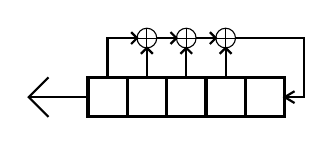
\begin{tikzpicture}[scale=0.05]
			\draw[black,very thick] (30,30) -- (30,40) -- (40,40) -- (40,30) -- (30,30) -- (30,40);
			\draw[black,thick] (35,40) -- (35,50) -- (35,50) -- (37.5,50);
			\draw[black,very thick] (40,30) -- (40,40) -- (50,40) -- (50,30) -- (40,30) -- (40,40);
			\draw[black,thick] (45,40) -- (45,47.5);
			\draw[black,thick] (43.5,46) -- (45,47.5) -- (46.5,46);
			\draw[black,thick] (37.5,50) -- (42.5,50);
			\draw[black,thick] (41,51.5) -- (42.5,50) -- (41,48.5);
			\draw (45,50) circle [radius=2.5];
			\draw[black] (42.5,50) -- (47.5,50);
			\draw[black] (45,47.5) -- (45,52.5);
			\draw[black,very thick] (50,30) -- (50,40) -- (60,40) -- (60,30) -- (50,30) -- (50,40);
			\draw[black,thick] (55,40) -- (55,47.5);
			\draw[black,thick] (53.5,46) -- (55,47.5) -- (56.5,46);
			\draw[black,thick] (47.5,50) -- (52.5,50);
			\draw[black,thick] (51,51.5) -- (52.5,50) -- (51,48.5);
			\draw (55,50) circle [radius=2.5];
			\draw[black] (52.5,50) -- (57.5,50);
			\draw[black] (55,47.5) -- (55,52.5);
			\draw[black,very thick] (60,30) -- (60,40) -- (70,40) -- (70,30) -- (60,30) -- (60,40);
			\draw[black,thick] (65,40) -- (65,47.5);
			\draw[black,thick] (63.5,46) -- (65,47.5) -- (66.5,46);
			\draw[black,thick] (57.5,50) -- (62.5,50);
			\draw[black,thick] (61,51.5) -- (62.5,50) -- (61,48.5);
			\draw (65,50) circle [radius=2.5];
			\draw[black] (62.5,50) -- (67.5,50);
			\draw[black] (65,47.5) -- (65,52.5);
			\draw[black,very thick] (70,30) -- (70,40) -- (80,40) -- (80,30) -- (70,30) -- (70,40);
			\draw[black,thick] (67.5,50) -- (85,50) -- (85,35) -- (80,35);
			\draw[black,thick] (82.5,36.5) -- (80,35) -- (82.5,33.5);
			\draw[black,thick] (30,35) -- (15,35);
			\draw[black,thick] (20,30) -- (15,35) -- (20,40);
		\end{tikzpicture}
	\end{center}
	\item Теперь, когда характеристический полином известен, восстанавливаем состояния регистра по последним 5 выходам:
	\begin{itemize}\itemsep1pt \parskip0pt \parsep0pt
		\item $\left(b_{5}, b_{4}, b_{3}, b_{2}, b_{1}\right) = \left(0, 0, 0, 0, 1\right)$. Сумма: $b_0 = b_{5} \oplus b_{4} \oplus b_{3} \oplus b_{2}=0 \oplus 0 \oplus 0 \oplus 0=0$. Следующее состояние $\left(0, 0, 0, 1, 0\right)$, а текущий выход $b_{5}=0$.
		\item $\left(b_{5}, b_{4}, b_{3}, b_{2}, b_{1}\right) = \left(0, 0, 0, 1, 0\right)$. Сумма: $b_0 = b_{5} \oplus b_{4} \oplus b_{3} \oplus b_{2}=0 \oplus 0 \oplus 0 \oplus 1=1$. Следующее состояние $\left(0, 0, 1, 0, 1\right)$, а текущий выход $b_{5}=0$.
		\item $\left(b_{5}, b_{4}, b_{3}, b_{2}, b_{1}\right) = \left(0, 0, 1, 0, 1\right)$. Сумма: $b_0 = b_{5} \oplus b_{4} \oplus b_{3} \oplus b_{2}=0 \oplus 0 \oplus 1 \oplus 0=1$. Следующее состояние $\left(0, 1, 0, 1, 1\right)$, а текущий выход $b_{5}=0$.
		\item $\left(b_{5}, b_{4}, b_{3}, b_{2}, b_{1}\right) = \left(0, 1, 0, 1, 1\right)$. Сумма: $b_0 = b_{5} \oplus b_{4} \oplus b_{3} \oplus b_{2}=0 \oplus 1 \oplus 0 \oplus 1=0$. Следующее состояние $\left(1, 0, 1, 1, 0\right)$, а текущий выход $b_{5}=0$.
		\item $\left(b_{5}, b_{4}, b_{3}, b_{2}, b_{1}\right) = \left(1, 0, 1, 1, 0\right)$. Сумма: $b_0 = b_{5} \oplus b_{4} \oplus b_{3} \oplus b_{2}=1 \oplus 0 \oplus 1 \oplus 1=1$. Следующее состояние $\left(0, 1, 1, 0, 1\right)$, а текущий выход $b_{5}=1$.
	\end{itemize}
	\item Следующие итерации, дающие нужный ответ:
	\begin{itemize}\itemsep1pt \parskip0pt \parsep0pt
		\item $\left(b_{5}, b_{4}, b_{3}, b_{2}, b_{1}\right) = \left(0, 1, 1, 0, 1\right)$. Сумма: $b_0 = b_{5} \oplus b_{4} \oplus b_{3} \oplus b_{2}=0 \oplus 1 \oplus 1 \oplus 0=0$. Следующее состояние $\left(1, 1, 0, 1, 0\right)$, а текущий выход $b_{5}=0$.
		\item $\left(b_{5}, b_{4}, b_{3}, b_{2}, b_{1}\right) = \left(1, 1, 0, 1, 0\right)$. Сумма: $b_0 = b_{5} \oplus b_{4} \oplus b_{3} \oplus b_{2}=1 \oplus 1 \oplus 0 \oplus 1=1$. Следующее состояние $\left(1, 0, 1, 0, 1\right)$, а текущий выход $b_{5}=1$.
		\item $\left(b_{5}, b_{4}, b_{3}, b_{2}, b_{1}\right) = \left(1, 0, 1, 0, 1\right)$. Сумма: $b_0 = b_{5} \oplus b_{4} \oplus b_{3} \oplus b_{2}=1 \oplus 0 \oplus 1 \oplus 0=0$. Следующее состояние $\left(0, 1, 0, 1, 0\right)$, а текущий выход $b_{5}=1$.
		\item $\left(b_{5}, b_{4}, b_{3}, b_{2}, b_{1}\right) = \left(0, 1, 0, 1, 0\right)$. Сумма: $b_0 = b_{5} \oplus b_{4} \oplus b_{3} \oplus b_{2}=0 \oplus 1 \oplus 0 \oplus 1=0$. Следующее состояние $\left(1, 0, 1, 0, 0\right)$, а текущий выход $b_{5}=0$.
		\item $\left(b_{5}, b_{4}, b_{3}, b_{2}, b_{1}\right) = \left(1, 0, 1, 0, 0\right)$. Сумма: $b_0 = b_{5} \oplus b_{4} \oplus b_{3} \oplus b_{2}=1 \oplus 0 \oplus 1 \oplus 0=0$. Следующее состояние $\left(0, 1, 0, 0, 0\right)$, а текущий выход $b_{5}=1$.
		\end{itemize}
	\item Итого ответ на вторую часть задачи: $0, 1, 1, 0, 1$.
	\item Краткое оформление второй части задачи можно увидеть в таблице~\ref{table:task-lfsr-2-short-solution}. Таблица заполняется сверху вниз. Столбцы таблицы связаны формулой $b_{5} \oplus b_{4} \oplus b_{3} \oplus b_{2} = b_0 $. В первой строке записаны первые 5 бит полученной последовательности. Выполняя последовательно операции над регистром мы получим все следующие биты. Начать заполнение таблицы можно со строчки $\overrightarrow s_{6}$ (то есть с последних 5 бит, данных в условии задачи), строки выше приведены для возможности (само)контроля студента. Ответом являются последние 5 бит в первом столбце.
	\begin{table}[!thb]
		\centering
		\begin{tabular}{ l | c || c c c c c|| c }
		 & & $b_{5}$& $b_{4}$& $b_{3}$& $b_{2}$& $b_{1}$ & $b_0$ \\
		  \hline
		  $\overrightarrow {s_{0}}$ & 0 & 0 & 1 & 0 & 0 & 1& 1 \\
		  \hline
		  $\overrightarrow {s_{1}}$ & 1 & 1 & 0 & 0 & 1 & 1& 0 \\
		  $\overrightarrow {s_{2}}$ & 0 & 0 & 0 & 1 & 1 & 0& 0 \\
		  $\overrightarrow {s_{3}}$ & 0 & 0 & 1 & 1 & 0 & 0& 0 \\
		  $\overrightarrow {s_{4}}$ & 1 & 1 & 1 & 0 & 0 & 0& 0 \\
		  $\overrightarrow {s_{5}}$ & 1 & 1 & 0 & 0 & 0 & 0& 1 \\
		  \hline
		  $\overrightarrow {s_{6}}$ & 0 & 0 & 0 & 0 & 0 & 1& 0 \\
		  $\overrightarrow {s_{7}}$ & 0 & 0 & 0 & 0 & 1 & 0& 1 \\
		  $\overrightarrow {s_{8}}$ & 0 & 0 & 0 & 1 & 0 & 1& 1 \\
		  $\overrightarrow {s_{9}}$ & 0 & 0 & 1 & 0 & 1 & 1& 0 \\
		  $\overrightarrow {s_{10}}$ & 1 & 1 & 0 & 1 & 1 & 0& 1 \\
		  \hline
		  $\overrightarrow {s_{11}}$ & 0 & 0 & 1 & 1 & 0 & 1& 0 \\
		  $\overrightarrow {s_{12}}$ & 1 & 1 & 1 & 0 & 1 & 0& 1 \\
		  $\overrightarrow {s_{13}}$ & 1 & 1 & 0 & 1 & 0 & 1& 0 \\
		  $\overrightarrow {s_{14}}$ & 0 & 0 & 1 & 0 & 1 & 0& 0 \\
		  $\overrightarrow {s_{15}}$ & 1 & 1 & 0 & 1 & 0 & 0& 0 \\
		\hline
		\end{tabular}
		\caption{Краткое оформление решения второй части задачи \No\arabic{task-section}.\arabic{task-number} в виде таблицы}
		\label{table:task-lfsr-2-short-solution}
	\end{table}
\end{itemize}
\medbreak
\textbf{Ответ:} полином $m \left( x \right) = x^{5} + x^{4} + x^{3} + x^{2} + 1$; дальнейшая последовательность: $0, 1, 1, 0, 1$.

\section{Псевдопростые числа}
\tasksection

\tasknumber Проверить, являются ли числа 73, 95 свидетелями простоты числа 111 по Ферма.
\medbreak
\textbf{Ответ:} да; нет.
\bigbreak

\tasknumber Проверить, являются ли числа 74, 448, 640, 660, 719 свидетелями простоты числа 793 по Миллеру.
\medbreak
\textbf{Ответ:} да; да; нет; нет; да.
\bigbreak

\section{Криптосистема RSA}
\tasksection

\tasknumber Зашифровать сообщение по схеме RSA. Открытый ключ: $n = 323$; $e = 245$. Сообщение: $m = 307$.
\medbreak
\textbf{Ответ:} $c = 86$.
\bigbreak

\tasknumber Расшифровать сообщение по схеме RSA. Для генерации пары открытого и секретного ключа использовались числа: $p = 13$; $q = 17$. Открытая экспонента: $e = 91$. Зашифрованное сообщение: $c = 196$.
\medbreak
\textbf{Ответ:} $d = 19$; $m = 66$.
\bigbreak

\tasknumber Расшифровать сообщение по схеме RSA. Открытый ключ: $n = 85$; $e = 15$. Зашифрованное сообщение: $c = 32$.
\medbreak
\textbf{Ответ:} $p = 5$; $q = 17$; $d = 47$; $m = 8$.
\bigbreak

\tasknumber Подписать сообщение по схеме RSA. Закрытый ключ: $n = 437$; $d = 181$. Сообщение: $m = 84$.
\medbreak
\textbf{Ответ:} $s = 122$.
\bigbreak

\tasknumber Подписать сообщение по схеме RSA. Открытый ключ: $n = 253$; $e = 159$. Сообщение: $m = 193$.
\medbreak
\textbf{Ответ:} $n = 11 \cdot 23$; $d = 119$; $s = 2$.

\section{Криптосистема Эль-Гамаля}
\tasksection

\tasknumber Зашифровать сообщение по схеме Эль-Гамаля. Открытый ключ: $p = 29$; $g = 10$; $y = 8$. Секретный ключ: $x = 5$. Сообщение: $M = 4$. Использовать следующий случайный параметр для шифрования: $k = 5$.
\medbreak
\textbf{Ответ:} $c = (a; b) = (8; 21)$.
\bigbreak

\tasknumber Расшифровать сообщение по схеме Эль-Гамаля. Открытый ключ: $p = 23$; $g = 5$; $y = 9$. Секретный ключ: $x = 10$. Зашифрованное сообщение: $\left( 10, 18\right)$.
\medbreak
\textbf{Ответ:} $m = 4$.
\bigbreak

\tasknumber Расшифровать сообщение по схеме Эль-Гамаля. Открытый ключ: $p = 29$; $g = 15$; $y = 28$. Зашифрованное сообщение: $\left( 10, 23\right)$.
\medbreak
\textbf{Ответ:} $x = 14$; $m = 6$.
\bigbreak

\tasknumber Проверить подпись по схеме Эль-Гамаля. Открытый ключ: $p = 29$; $g = 14$; $y = 7$. Сообщение: $m = 7$. Подпись: $a = 19$;  $b = 19$.
\medbreak
\textbf{Ответ:} $12 = 12$.
\bigbreak

\tasknumber Подписать сообщение по схеме Эль-Гамаля. Открытый ключ: $p = 23$; $g = 20$; $y = 17$. Сообщение: $m = 4$. Использовать следующий случайный параметр для создания подписи: $k = 7$.
\medbreak
\textbf{Ответ:} $x = 19$; $s = (a; b) = (21; 19)$.
\bigbreak

\section{Эллиптические кривые}
\tasksection

\tasknumber Для точки A (8; 6), принадлежащей группе точек эллиптической кривой $y^2 = x^3 - 9x - 13$ над конечным полем $\mathbb{F}_{17}$, найти координаты точек $B = 2 \times A = A + A$ и $C = 3 \times A = A + A + A$.
\medbreak
\textbf{Ответ:} $(3; 15)$, $(14; 15)$.
\bigbreak

\tasknumber Найти группу точек (перечислить все точки) эллиптической кривой $y^2 = x^3 - 2 x - 10$ над конечным полем $\mathbb{F}_{13}$.
\medbreak
\textbf{Решение:} получение группы точек с помощью таблицы:\\
\begin{tabular}{|r|r|r|r|r|r|r|r|}
\hline
$x$ & $x^2$ & $x^3$ & $-2x$ & $-10$ & $y^2$ & $y_1$, $y_2$ & точки \\ 
\hline
$0$ & $0$ & $0$ & $-0$ & $-10$ & $3$ & $4$,$9$ &$(0; 4)$, $(0; 9)$ \\ 
$1$ & $1$ & $1$ & $-2$ & $-10$ & $2$ &  --- & --- \\ 
$2$ & $4$ & $8$ & $-4$ & $-10$ & $7$ &  --- & --- \\ 
$3$ & $9$ & $1$ & $-6$ & $-10$ & $11$ &  --- & --- \\ 
$4$ & $3$ & $12$ & $-8$ & $-10$ & $7$ &  --- & --- \\ 
$5$ & $12$ & $8$ & $-10$ & $-10$ & $1$ & $1$,$12$ &$(5; 1)$, $(5; 12)$ \\ 
$6$ & $10$ & $8$ & $-12$ & $-10$ & $12$ & $5$,$8$ &$(6; 5)$, $(6; 8)$ \\ 
$7$ & $10$ & $5$ & $-1$ & $-10$ & $7$ &  --- & --- \\ 
$8$ & $12$ & $5$ & $-3$ & $-10$ & $5$ &  --- & --- \\ 
$9$ & $3$ & $1$ & $-5$ & $-10$ & $12$ & $5$,$8$ &$(9; 5)$, $(9; 8)$ \\ 
$10$ & $9$ & $12$ & $-7$ & $-10$ & $8$ &  --- & --- \\ 
$11$ & $4$ & $5$ & $-9$ & $-10$ & $12$ & $5$,$8$ &$(11; 5)$, $(11; 8)$ \\ 
$12$ & $1$ & $12$ & $-11$ & $-10$ & $4$ & $2$,$11$ &$(12; 2)$, $(12; 11)$ \\ 
\hline
\end{tabular}
\medbreak
\textbf{Ответ:}
\begin{itemize}
\item Точки эллиптической кривой: [(0; 4), (0; 9), (5; 1), (5; 12), (6; 5), (6; 8), (9; 5), (9; 8), (11; 5), (11; 8), (12; 2), (12; 11), 0];
\item Размер группы точек: $13$.
\end{itemize}
\bigbreak

\tasknumber Для точки $\left(6; 9\right)$ определить, является ли она генератором всей группы точек кривой $y^2 = x^3 - 10 x - 7$ над конечным полем $\mathbb{F}_{17}$ или подгруппы. Перечислить точки генерируемой подгруппы (группы).
\medbreak
\textbf{Ответ:} точка $\left(6; 9\right)$ — генератор подгруппы размера 4: [(6; 9), (4; 0), (6; 8), 0].
\bigbreak

\tasknumber Вычислить электронную подпись сообщения $m=5$ по схеме ГОСТ Р 34.10-2012. Кривая $y^2 = x^3 - 3 x - 8$ над конечным полем $\mathbb{F}_{11}$. В качестве генератора используется точка G$\left(0; 5\right)$, размер циклической подгруппы -- $16$. Открытый ключ отправителя сообщения Q$\left(10; 4\right)$. Для генерации ЭП использовать случайный параметр $k=3$.
\medbreak
\textbf{Решение:}
\begin{itemize}
\item Используя формулу $Q = d \times G$, перебором находим, что $d = 5$.
\item $C = k \times G = 3 \times \left(0; 5\right) = \left(6; 5\right)$.
\item $r = x_C \bmod q = 6 \bmod 16 = 6$.
\item $e = m \bmod q = 5 \bmod 16 = 5$.
\item $s = ( r d + k e ) \bmod q = ( 6 \cdot 5 + 3 \cdot 5 ) \bmod 16 = 13$.
\end{itemize}
\medbreak
\textbf{Ответ:} подпись: $(x_c, s) = (6, 13)$.
\bigbreak

\section{Протоколы распространения ключей}
\tasksection

\tasknumber Алиса и Боб участвуют в группе распределения ключей по схеме Блома с модулем $p = 11$. Алисе выдан идентификатор $\overrightarrow{(5; 7)}$ и соответствующий ему закрытый ключ $\overrightarrow{(5; 8)}$. Вычислите общий сеансовый ключ Алисы и Боба, если открытый ключ Боба $\overrightarrow{(4; 3)}$. Найдите секретную матрицу доверенного центра, если известно, что закрытый ключ Боба -- $\overrightarrow{(1; 4)}$.
\medbreak
\textbf{Ответ:} $s = 0$. $\left( {\begin{array}{*{20}c}
   7 & 2  \\
   2 & 6  \\
\end{array}} \right)$ -- секретная матрица доверенного центра.
\bigbreak

\tasknumber Сгенерировать секретный сеансовый ключ для Алисы и Боба по протоколу Диффи~---~Хеллмана\index{протокол!Диффи~---~Хеллмана}. Общие параметры схемы: генератор 14 и модуль 17. Открытые ключи Алисы и Боба равны 8 и 5 соответственно.
\medbreak
\textbf{Решение и ответ:}
\begin{itemize}
\item Закрытый ключ Алисы: $a = \log_{g} A \bmod p = \log_{14} 8 \bmod 17 = 10$.
\item Закрытый ключ Боба: $b = \log_{g} B \bmod p = \log_{14} 5 \bmod 17 = 13$.
\item Генерация Алисой: $s = {B}^{a} \bmod p  = {5}^{10} \bmod 17 = 9$.
\item Генерация Бобом: $s = {A}^{b} \bmod p  = {8}^{13} \bmod 17 = 9$.
\end{itemize}

\section{Разделение секрета}
\tasksection

\tasknumber При разделении секрета по $(k, n)$-пороговой векторной схеме\index{схема!векторная} (схеме Блэкли\index{схема!Блэкли}) с модулем $p = 11$ получены 4 следа: $\left( {8, 1, 4} \right)$, $\left( {9, 8, 10} \right)$, $\left( {4, 2, 1} \right)$, $\left( {4, 7, 5} \right)$. Восстановите исходную точку и секрет, если известно, что это первая координата (x) точки.
\medbreak
\textbf{Ответ:} $M = 4$.
\bigbreak

\tasknumber Секрет был разделён по $(3, n)$-пороговой схеме Шамира\index{схема!Шамира} с модулем $p=11$. Известны четыре следа: $\left( {3, 9} \right)$, $\left( {4, 9} \right)$, $\left( {5, 10} \right)$, $\left( {6, 1} \right)$. Восстановить оптимальным способом исходный многочлен и секрет.
\medbreak
\textbf{Ответ:} исходный многочлен: $F\left( x \right) = ax^2  + bx + M = 6x^2  + 2x + 4$. Секретом является последний свободный многочлен $M = 4$.
\bigbreak

\tasknumber Используя эллиптическую кривую $y^2 = x^3 - 1x - 7$ над конечным полем $\mathbb{F}_{11}$, генератор $G(0; 2)$ и открытый ключ Боба $K_B(10; 9)$, Алиса сгенерировала разделяемый секрет (по схеме ECIES\index{схема!ECIES}) $S=P_x$ для последующего использования в качестве ключа шифрования и передала Бобу соответствующий секрету след $R(9; 8)$. Найдите секрет $S$, если закрытый ключ Боба $k_B = 6$.
\medbreak
\textbf{Ответ:} $P_x = 5$.

